\section{Introduction}

\hidenum
\begin{frame}[noframenumbering]
\frametitle{Contents}
 \tableofcontents[currentsection,hideothersubsections,sectionstyle=show/hide]
\end{frame}
\shownum

\subsection{Quick Overview of Parallel Hardware}

\begin{frame}
\begin{block}{Three Basic Flavors of Hardware}
    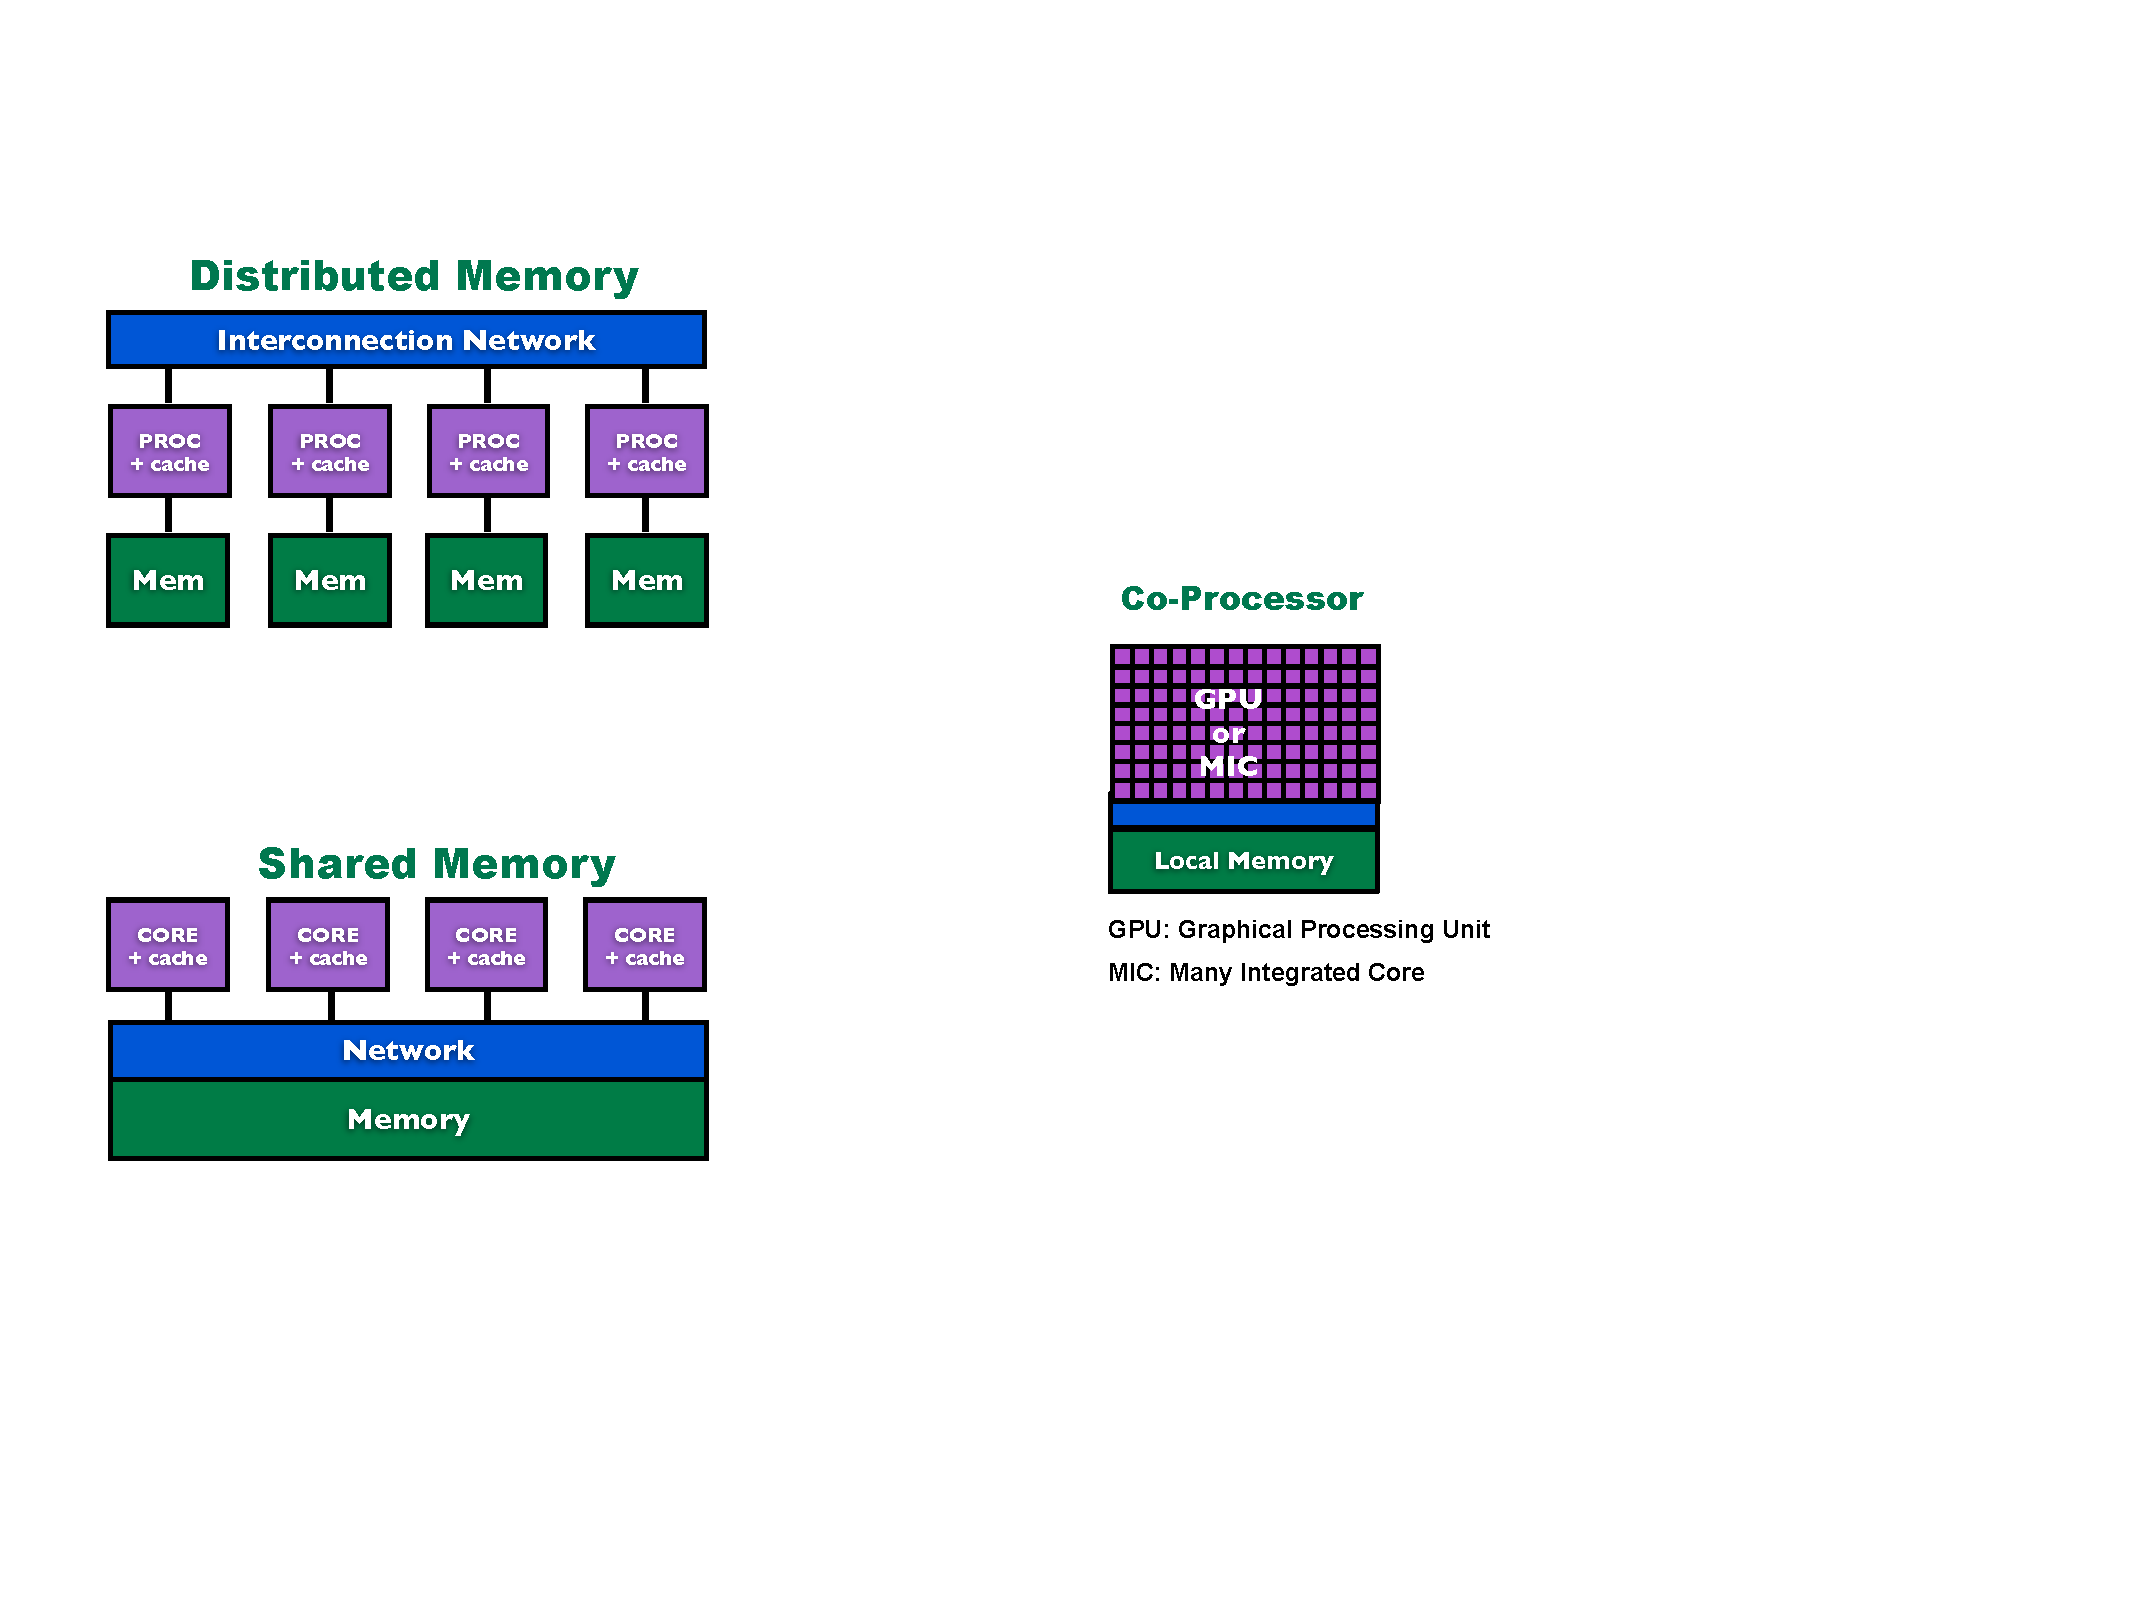
\includegraphics[width=0.95\textwidth]{../common/pics/ParallelHardware1.pdf}
\end{block}
\end{frame}

\begin{frame}
\begin{block}{Your Laptop or Desktop}
    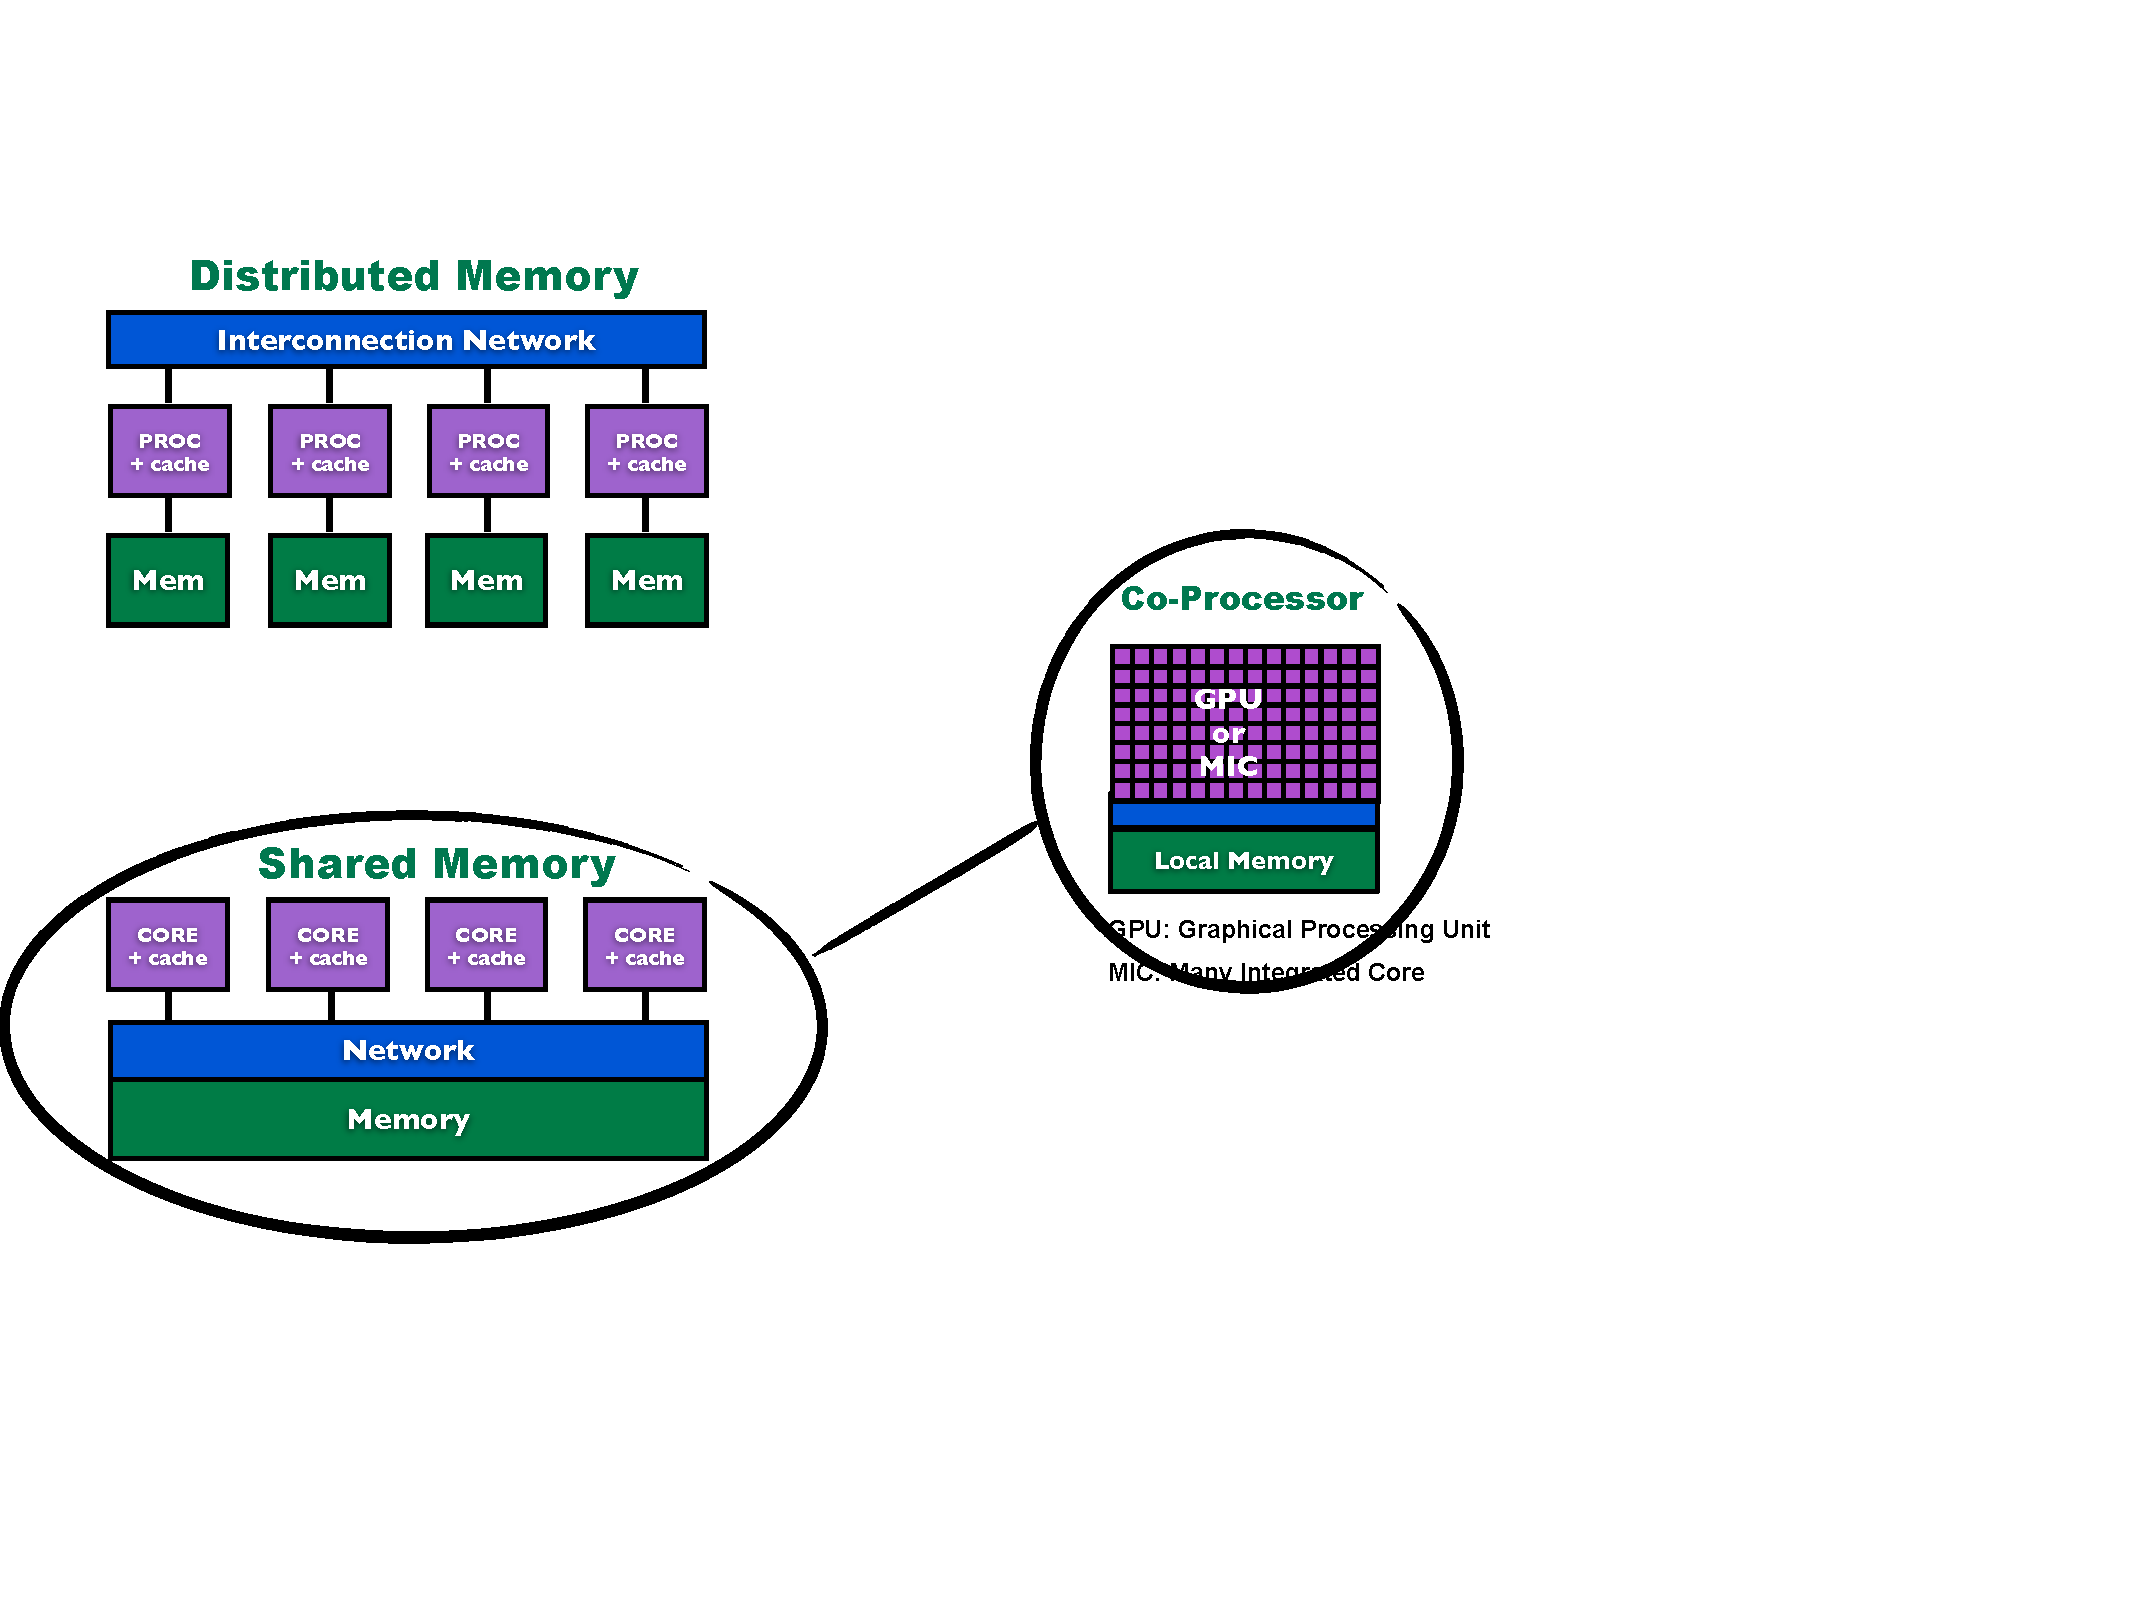
\includegraphics[width=0.95\textwidth]{../common/pics/ParallelHardware2.pdf}
\end{block}
\end{frame}

\begin{frame}
\begin{block}{A Server or Cluster}
    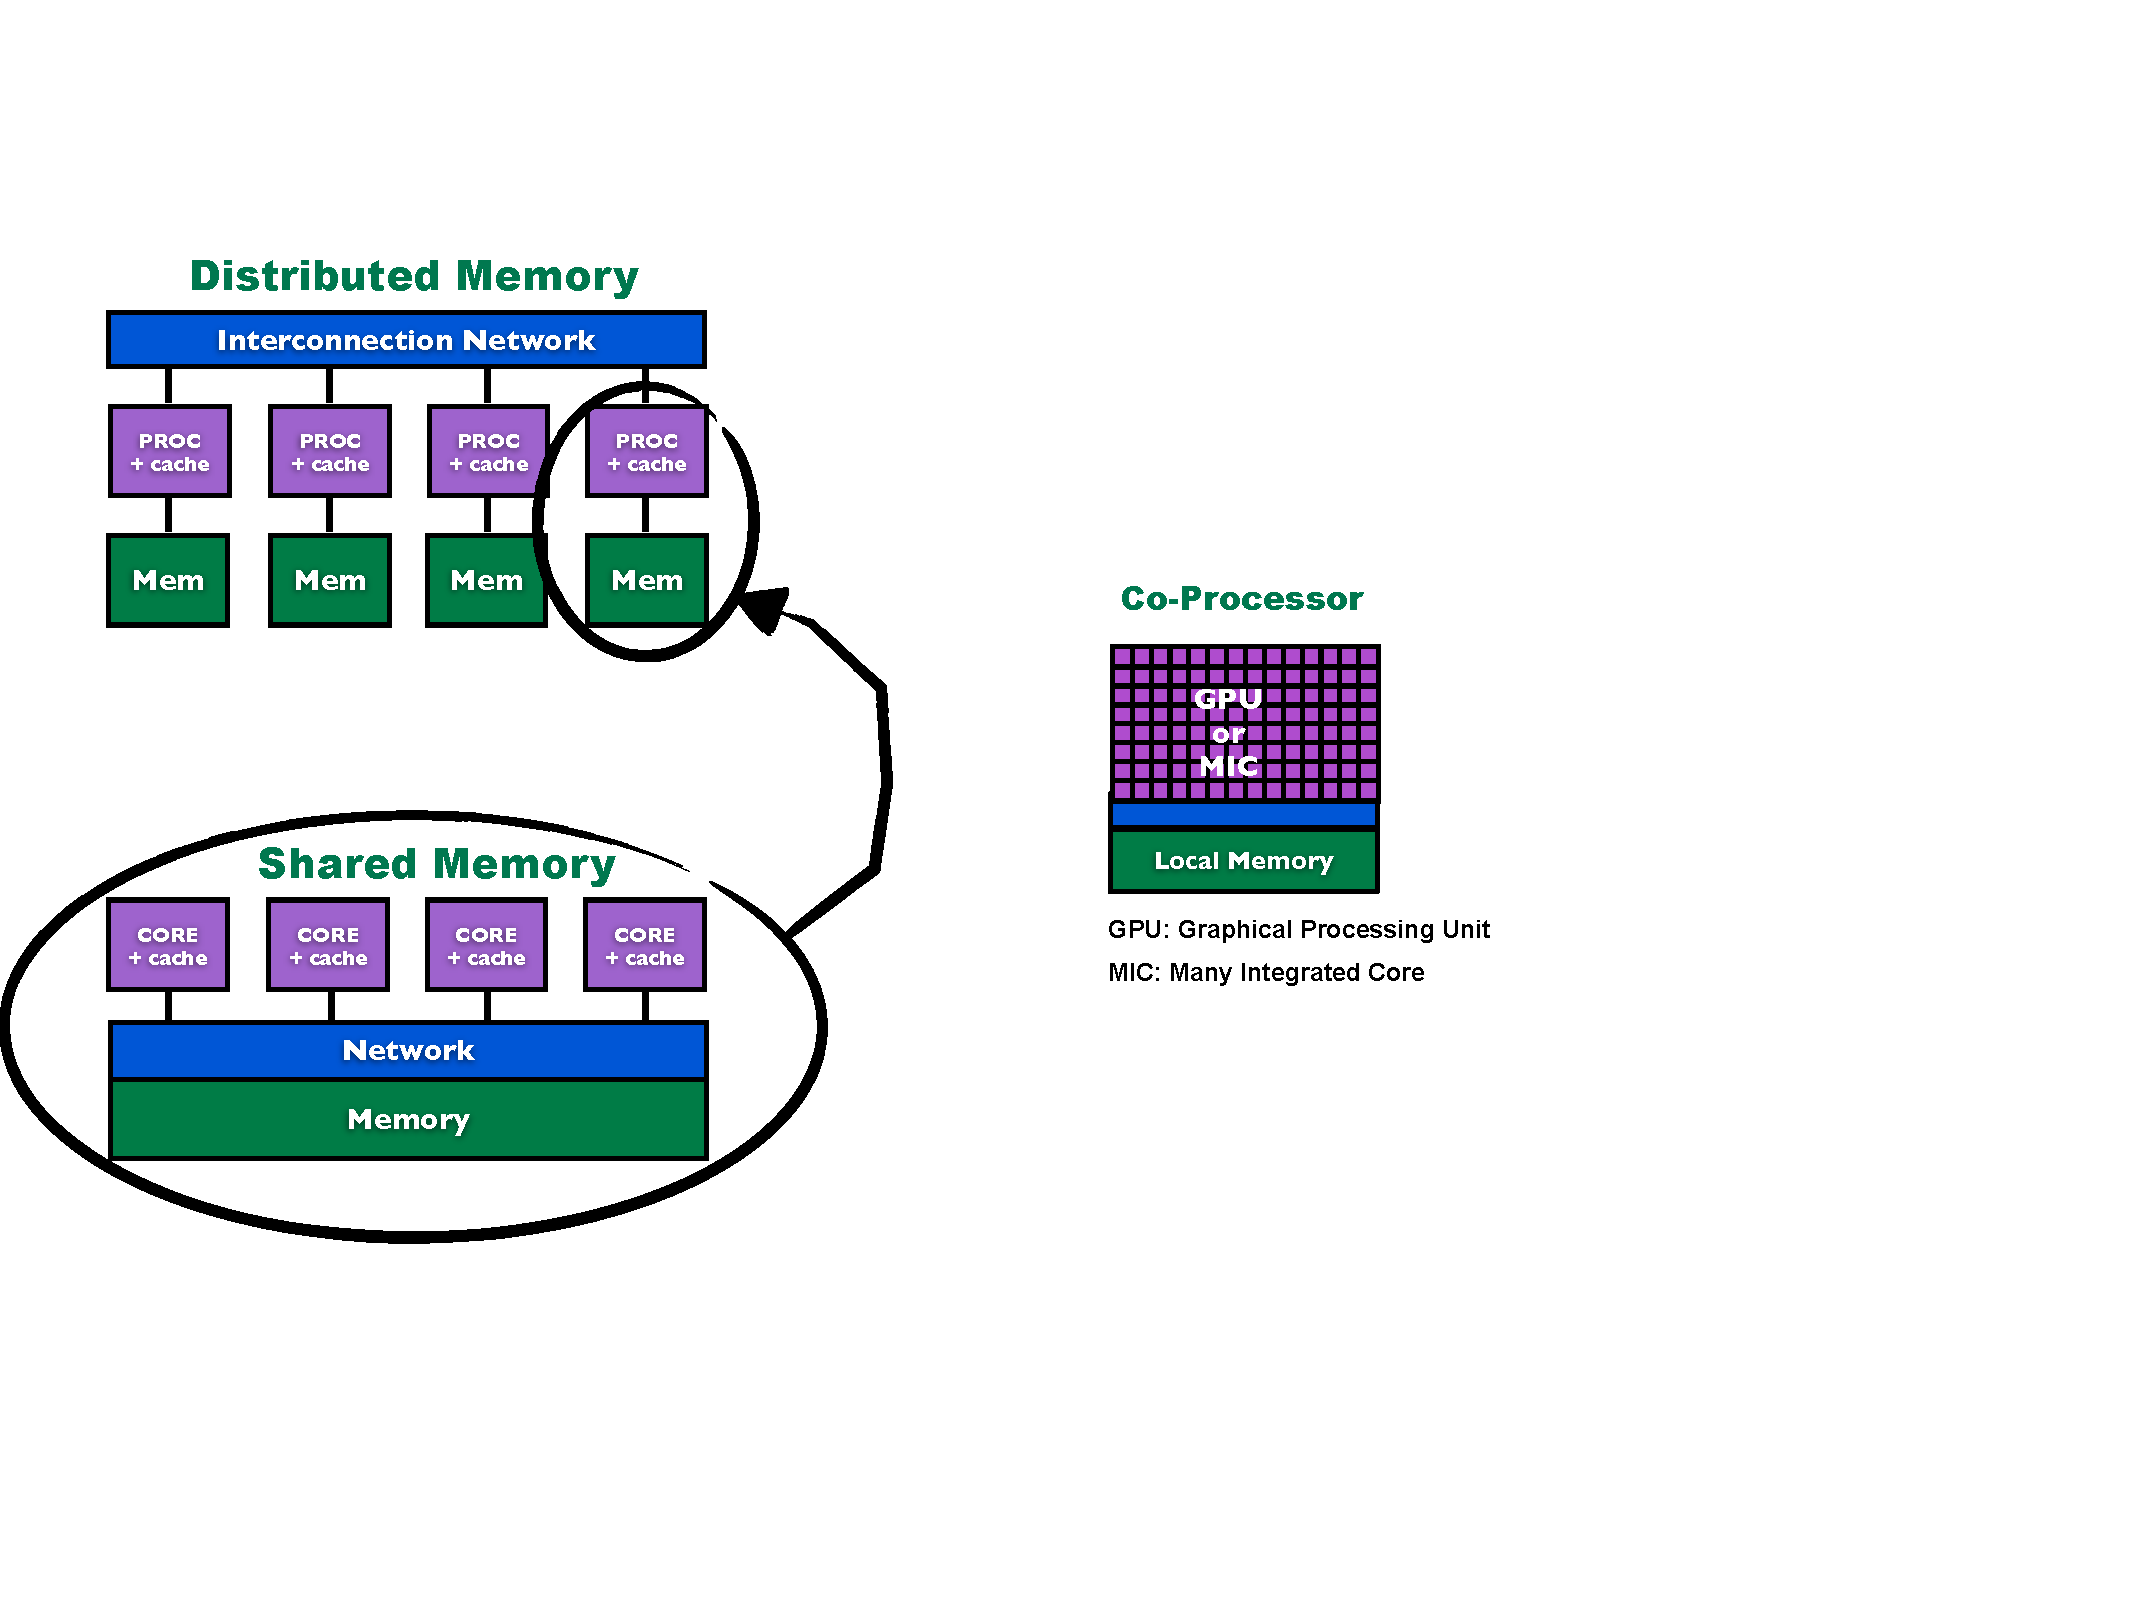
\includegraphics[width=0.95\textwidth]{../common/pics/ParallelHardware3.pdf}
\end{block}
\end{frame}

\begin{frame}
\begin{block}{Server to Supercomputer}
    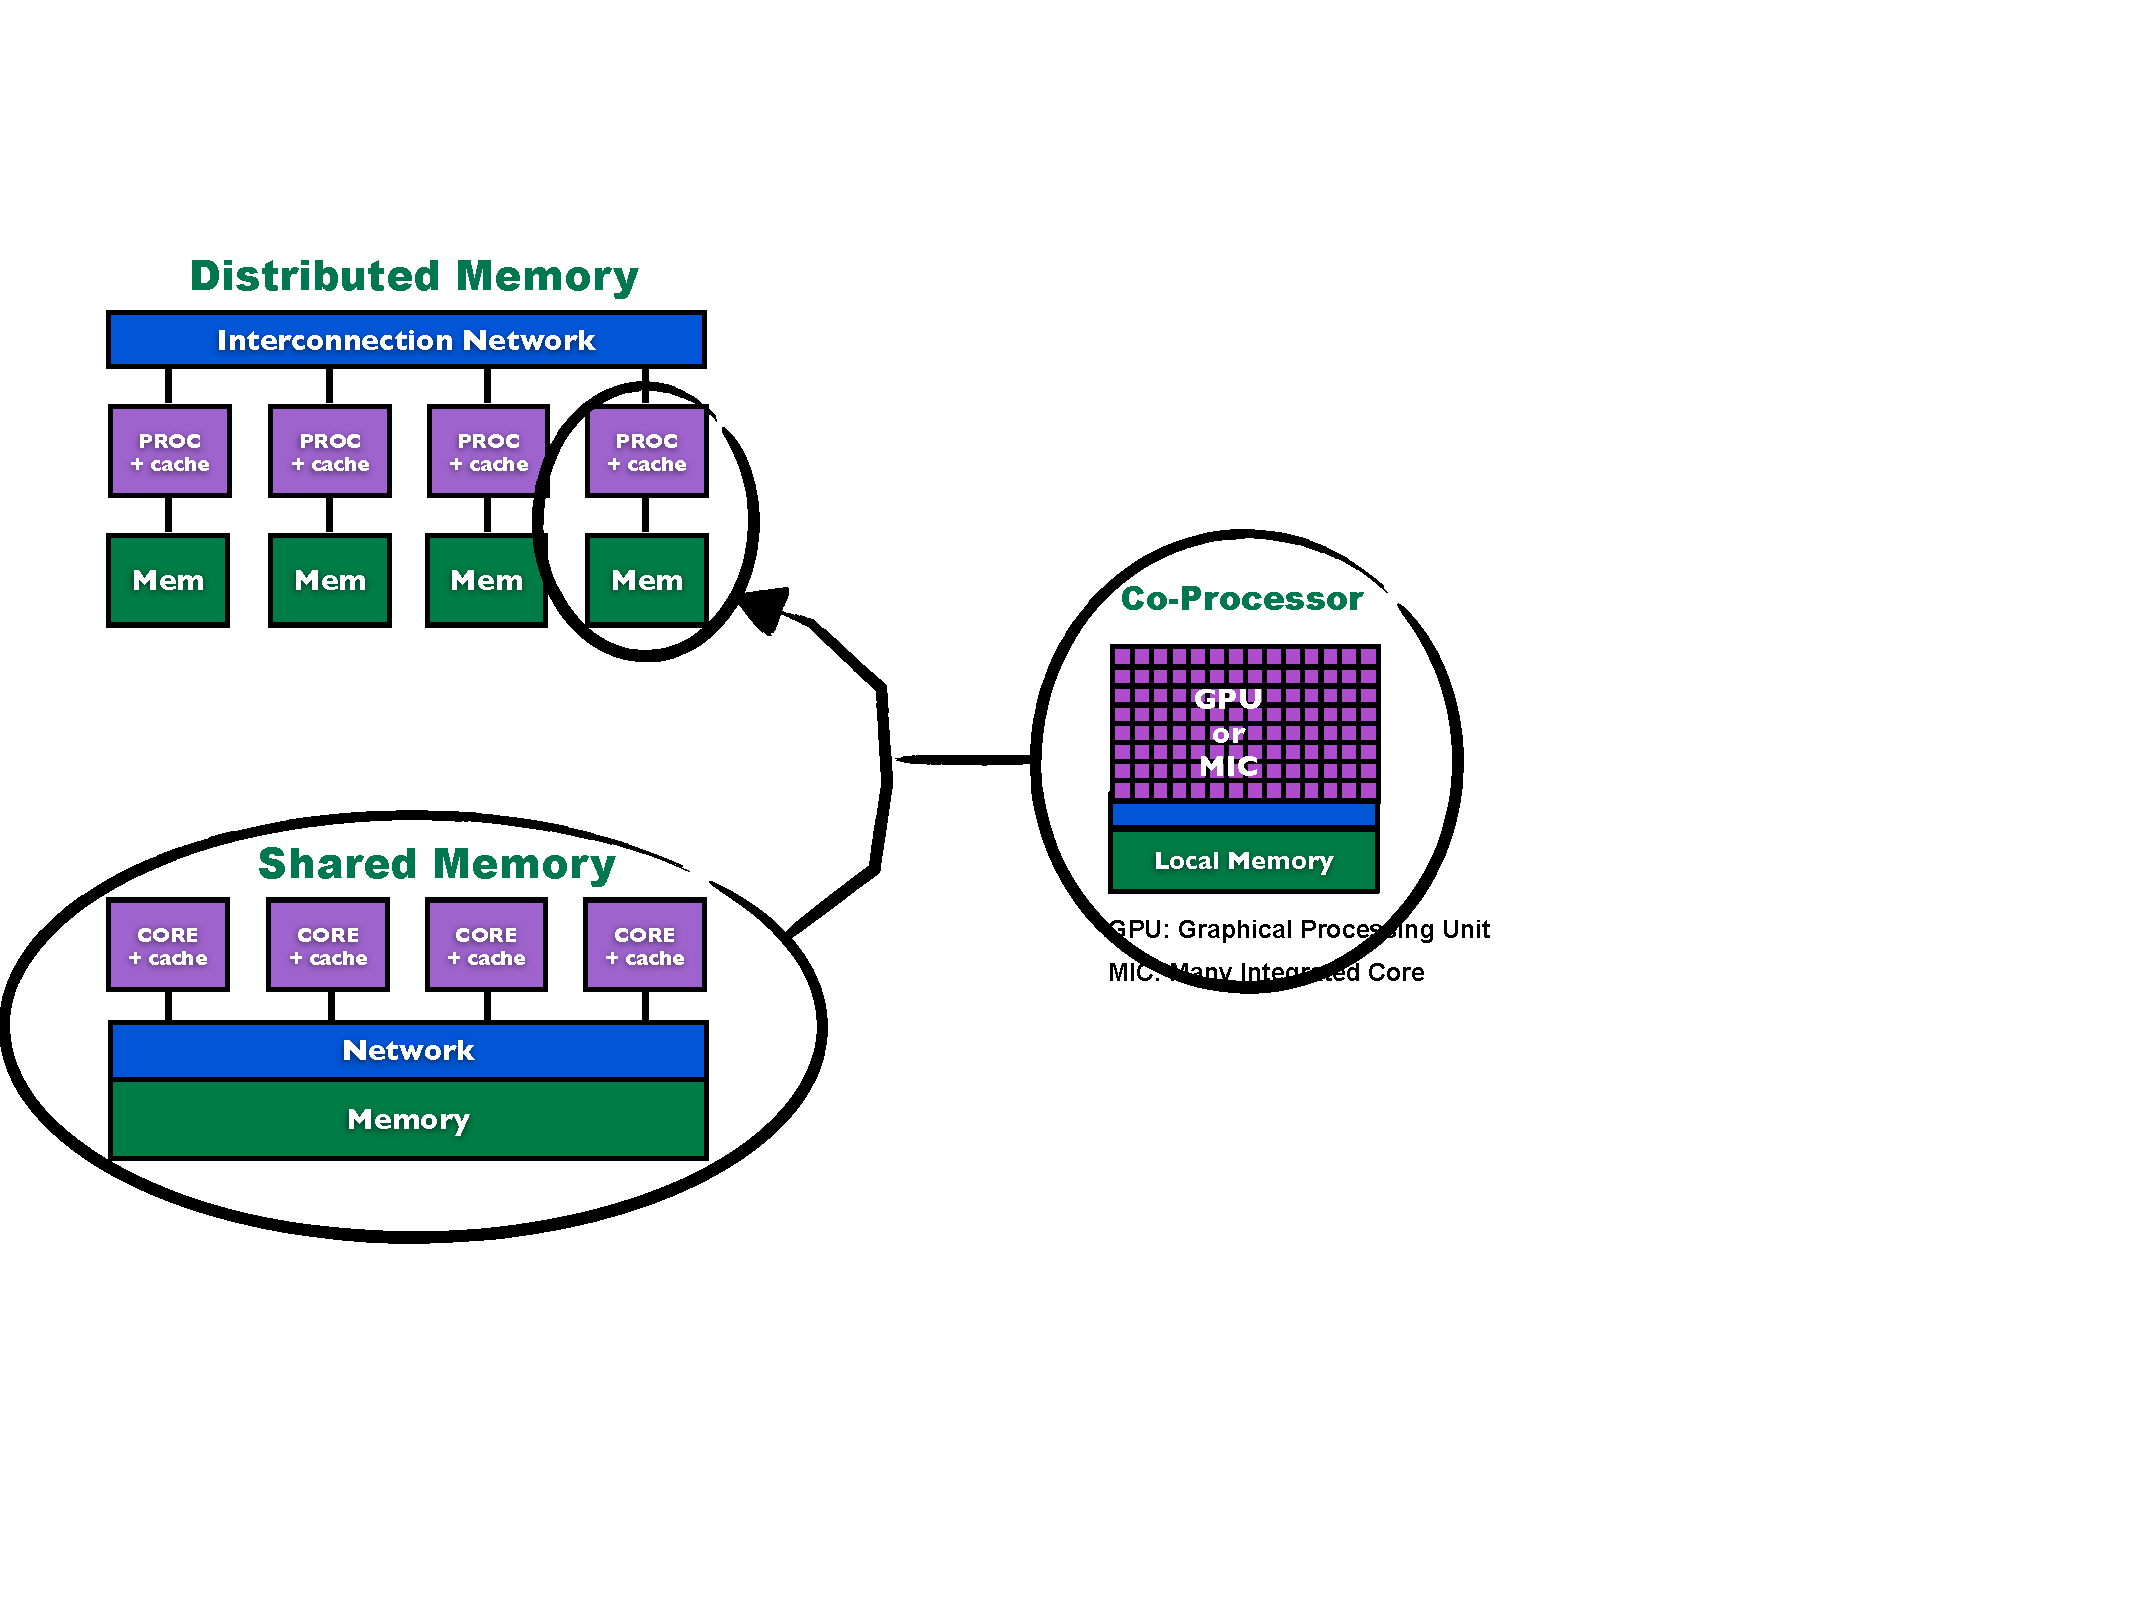
\includegraphics[width=0.95\textwidth]{../common/pics/ParallelHardware4.pdf}
\end{block}
\end{frame}

\begin{frame}
\begin{block}{Knowing the Right Words}
    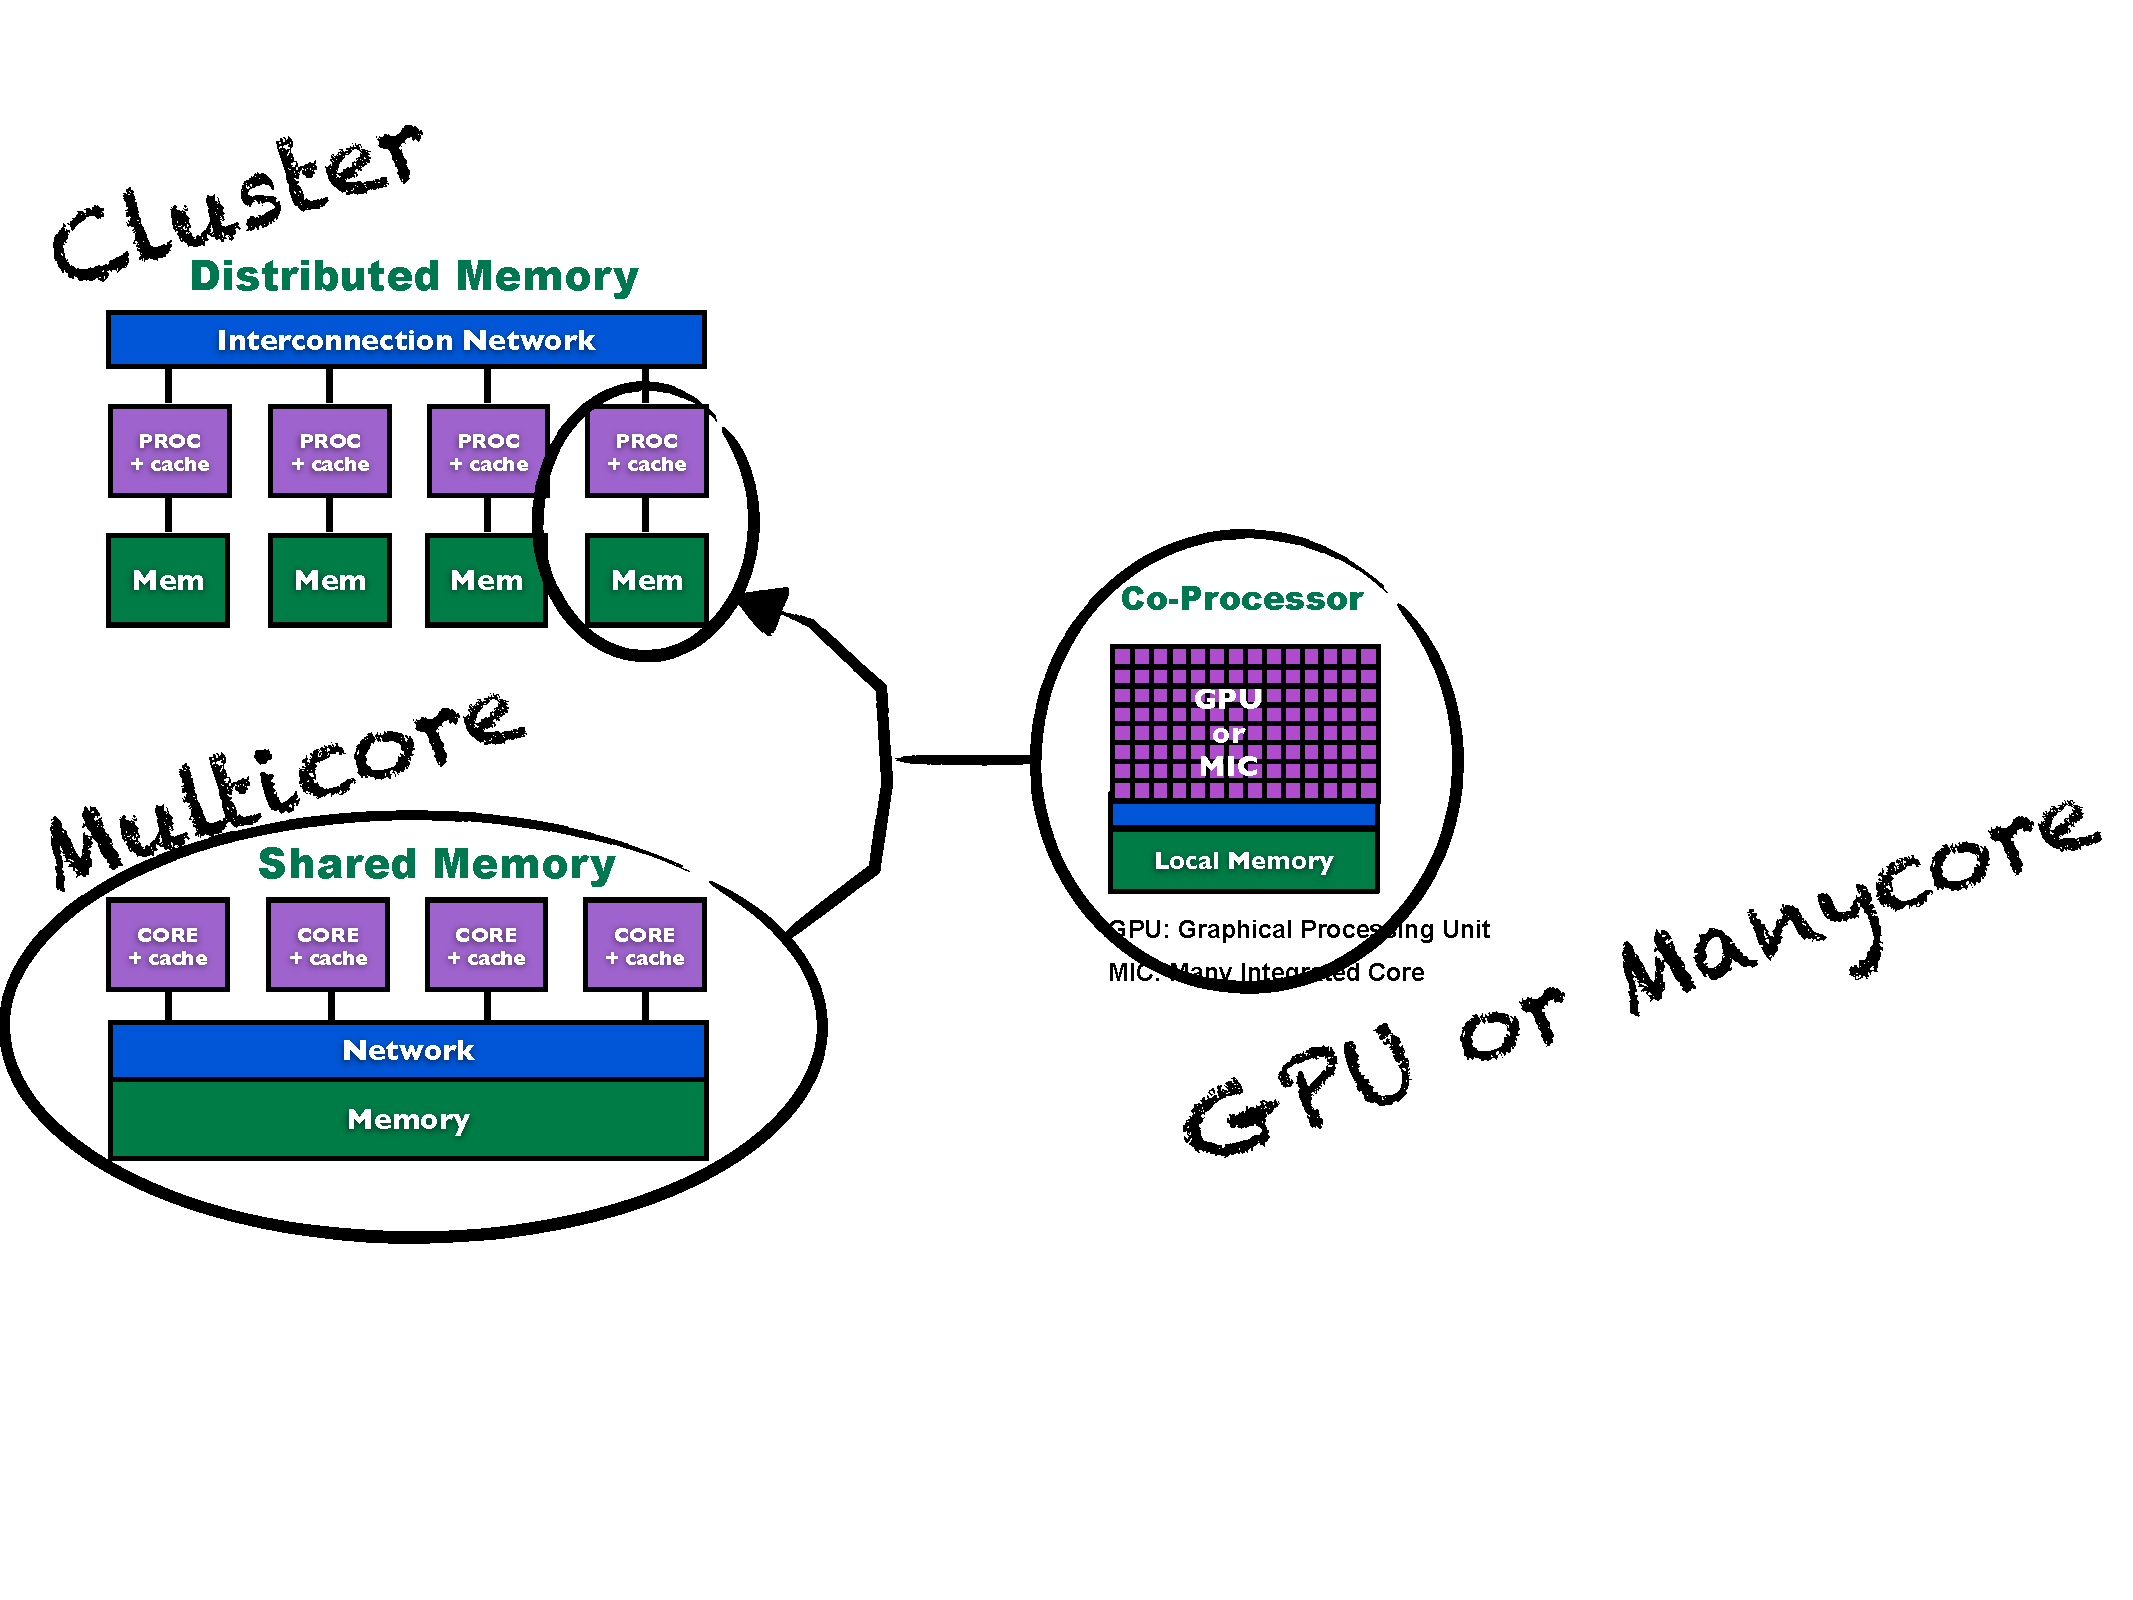
\includegraphics[width=0.95\textwidth]{../common/pics/ParallelHardware5.pdf}
\end{block}
\end{frame}

\begin{frame}
\begin{block}{``Native'' Programming Models and Tools}
    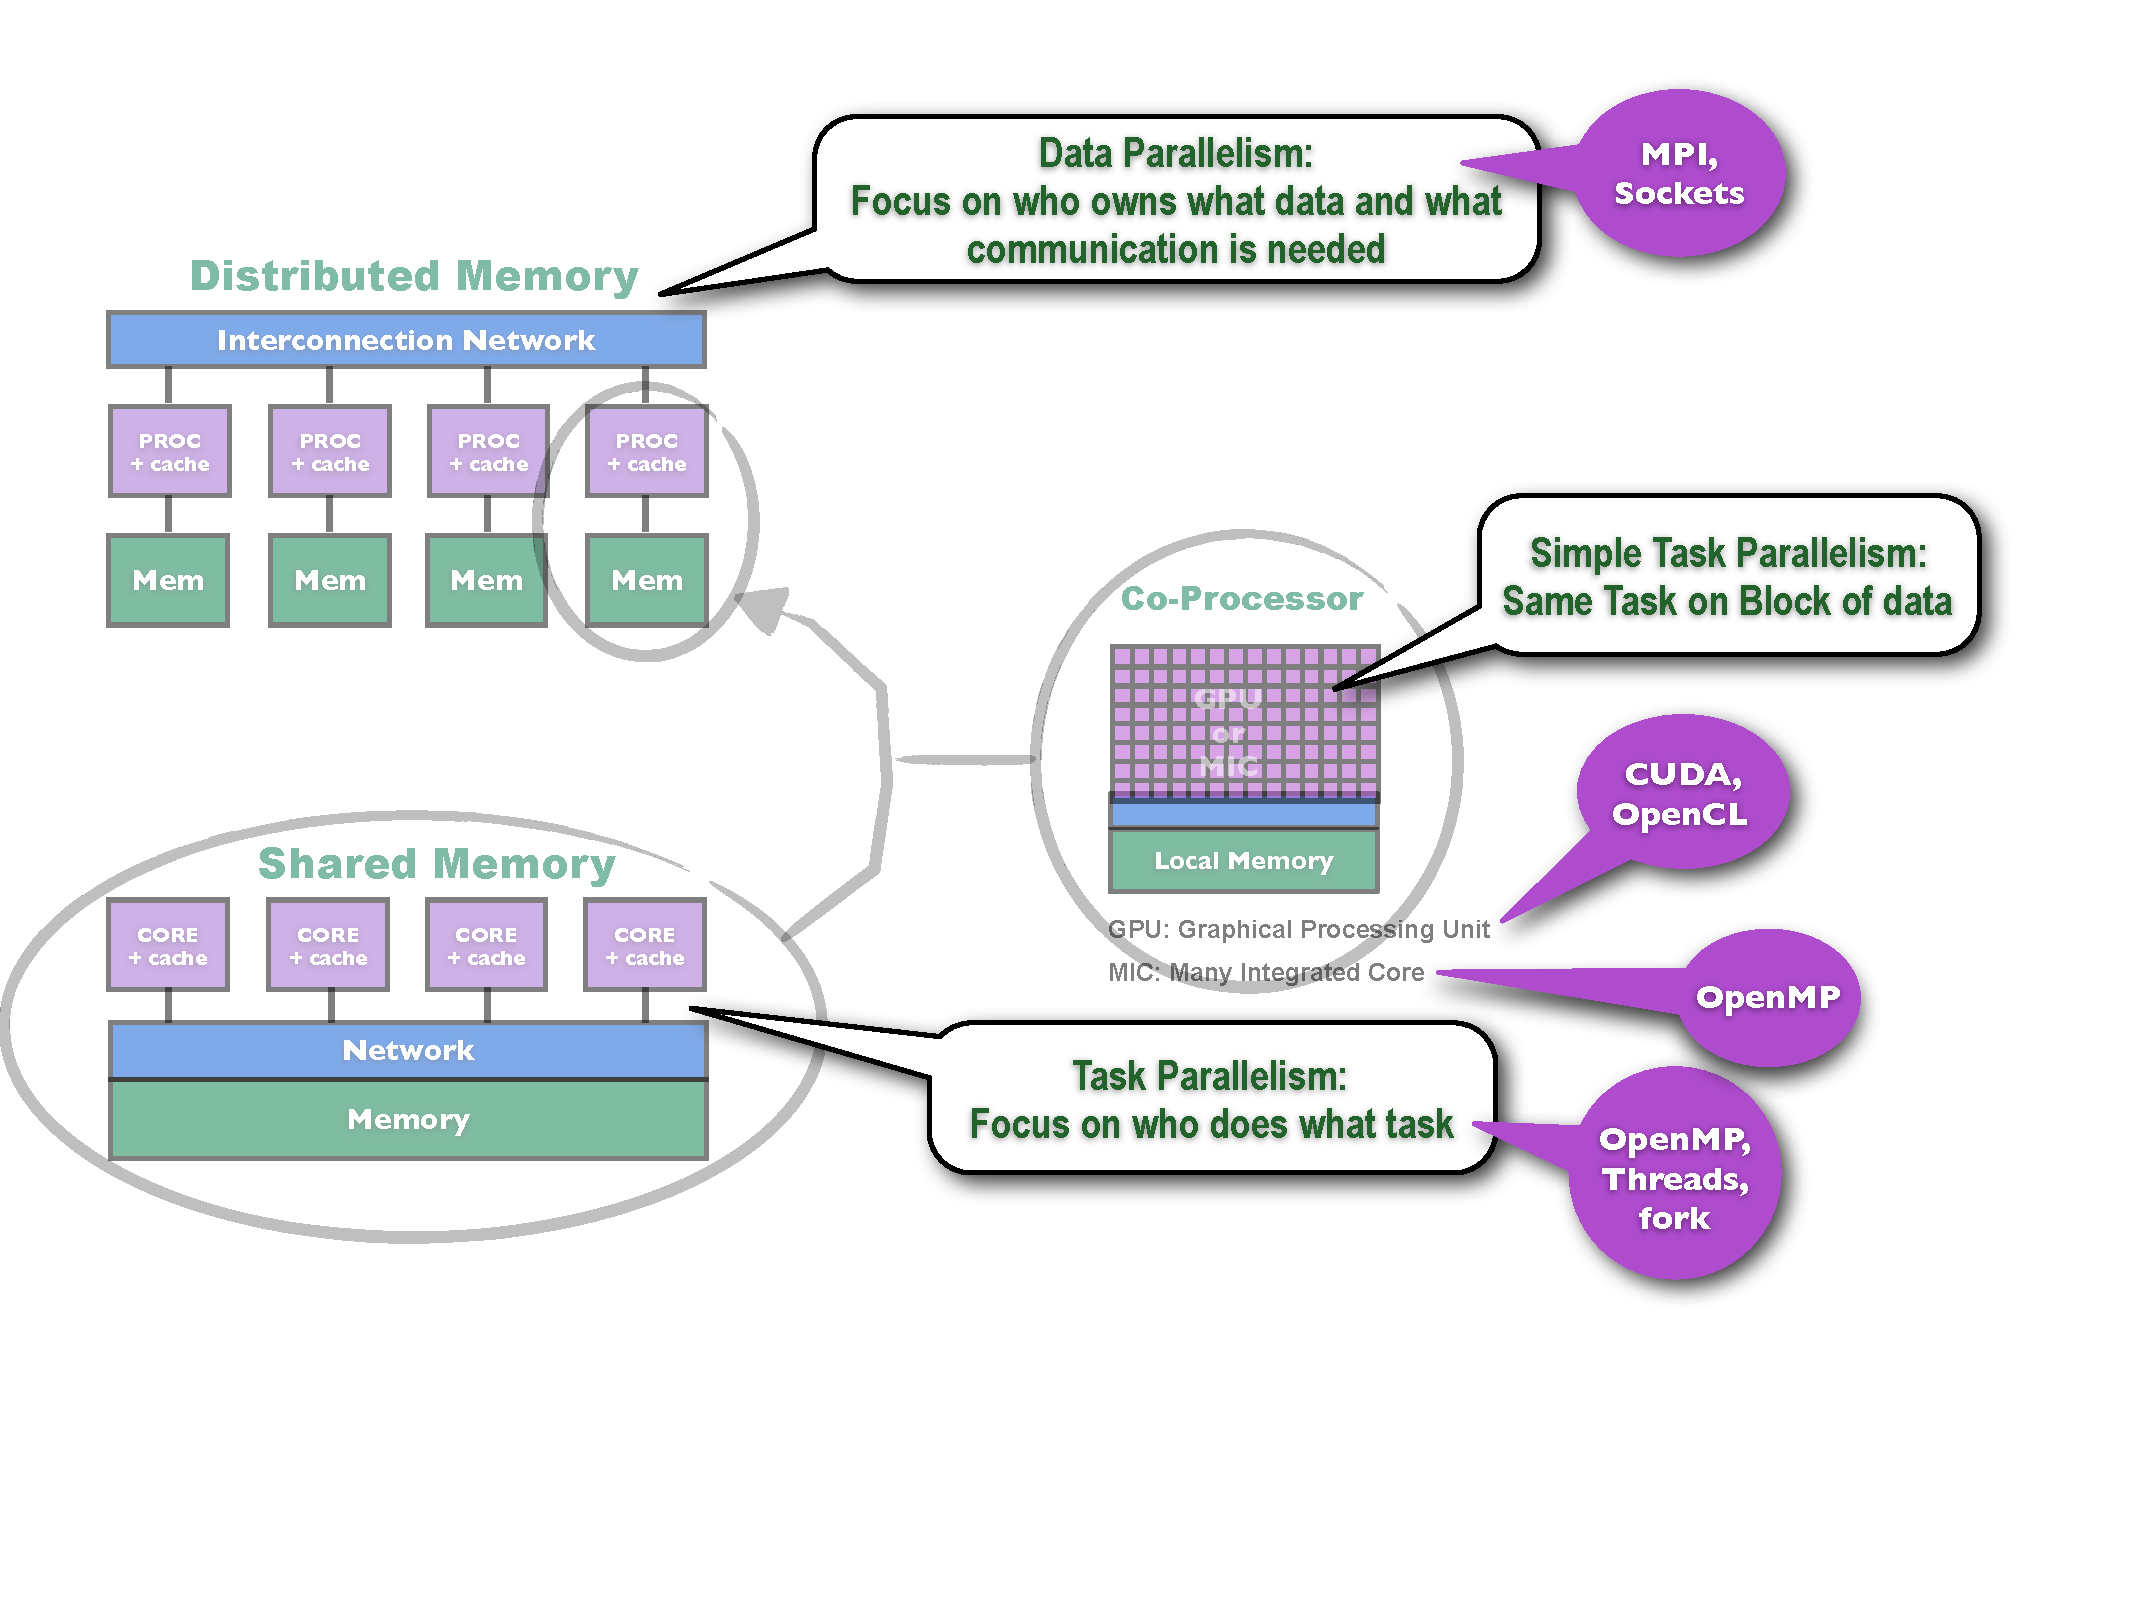
\includegraphics[width=0.95\textwidth]{../common/pics/ParallelHardware6.pdf}
\end{block}
\end{frame}

\begin{frame}
\begin{block}{R Interfaces to Native Tools}
    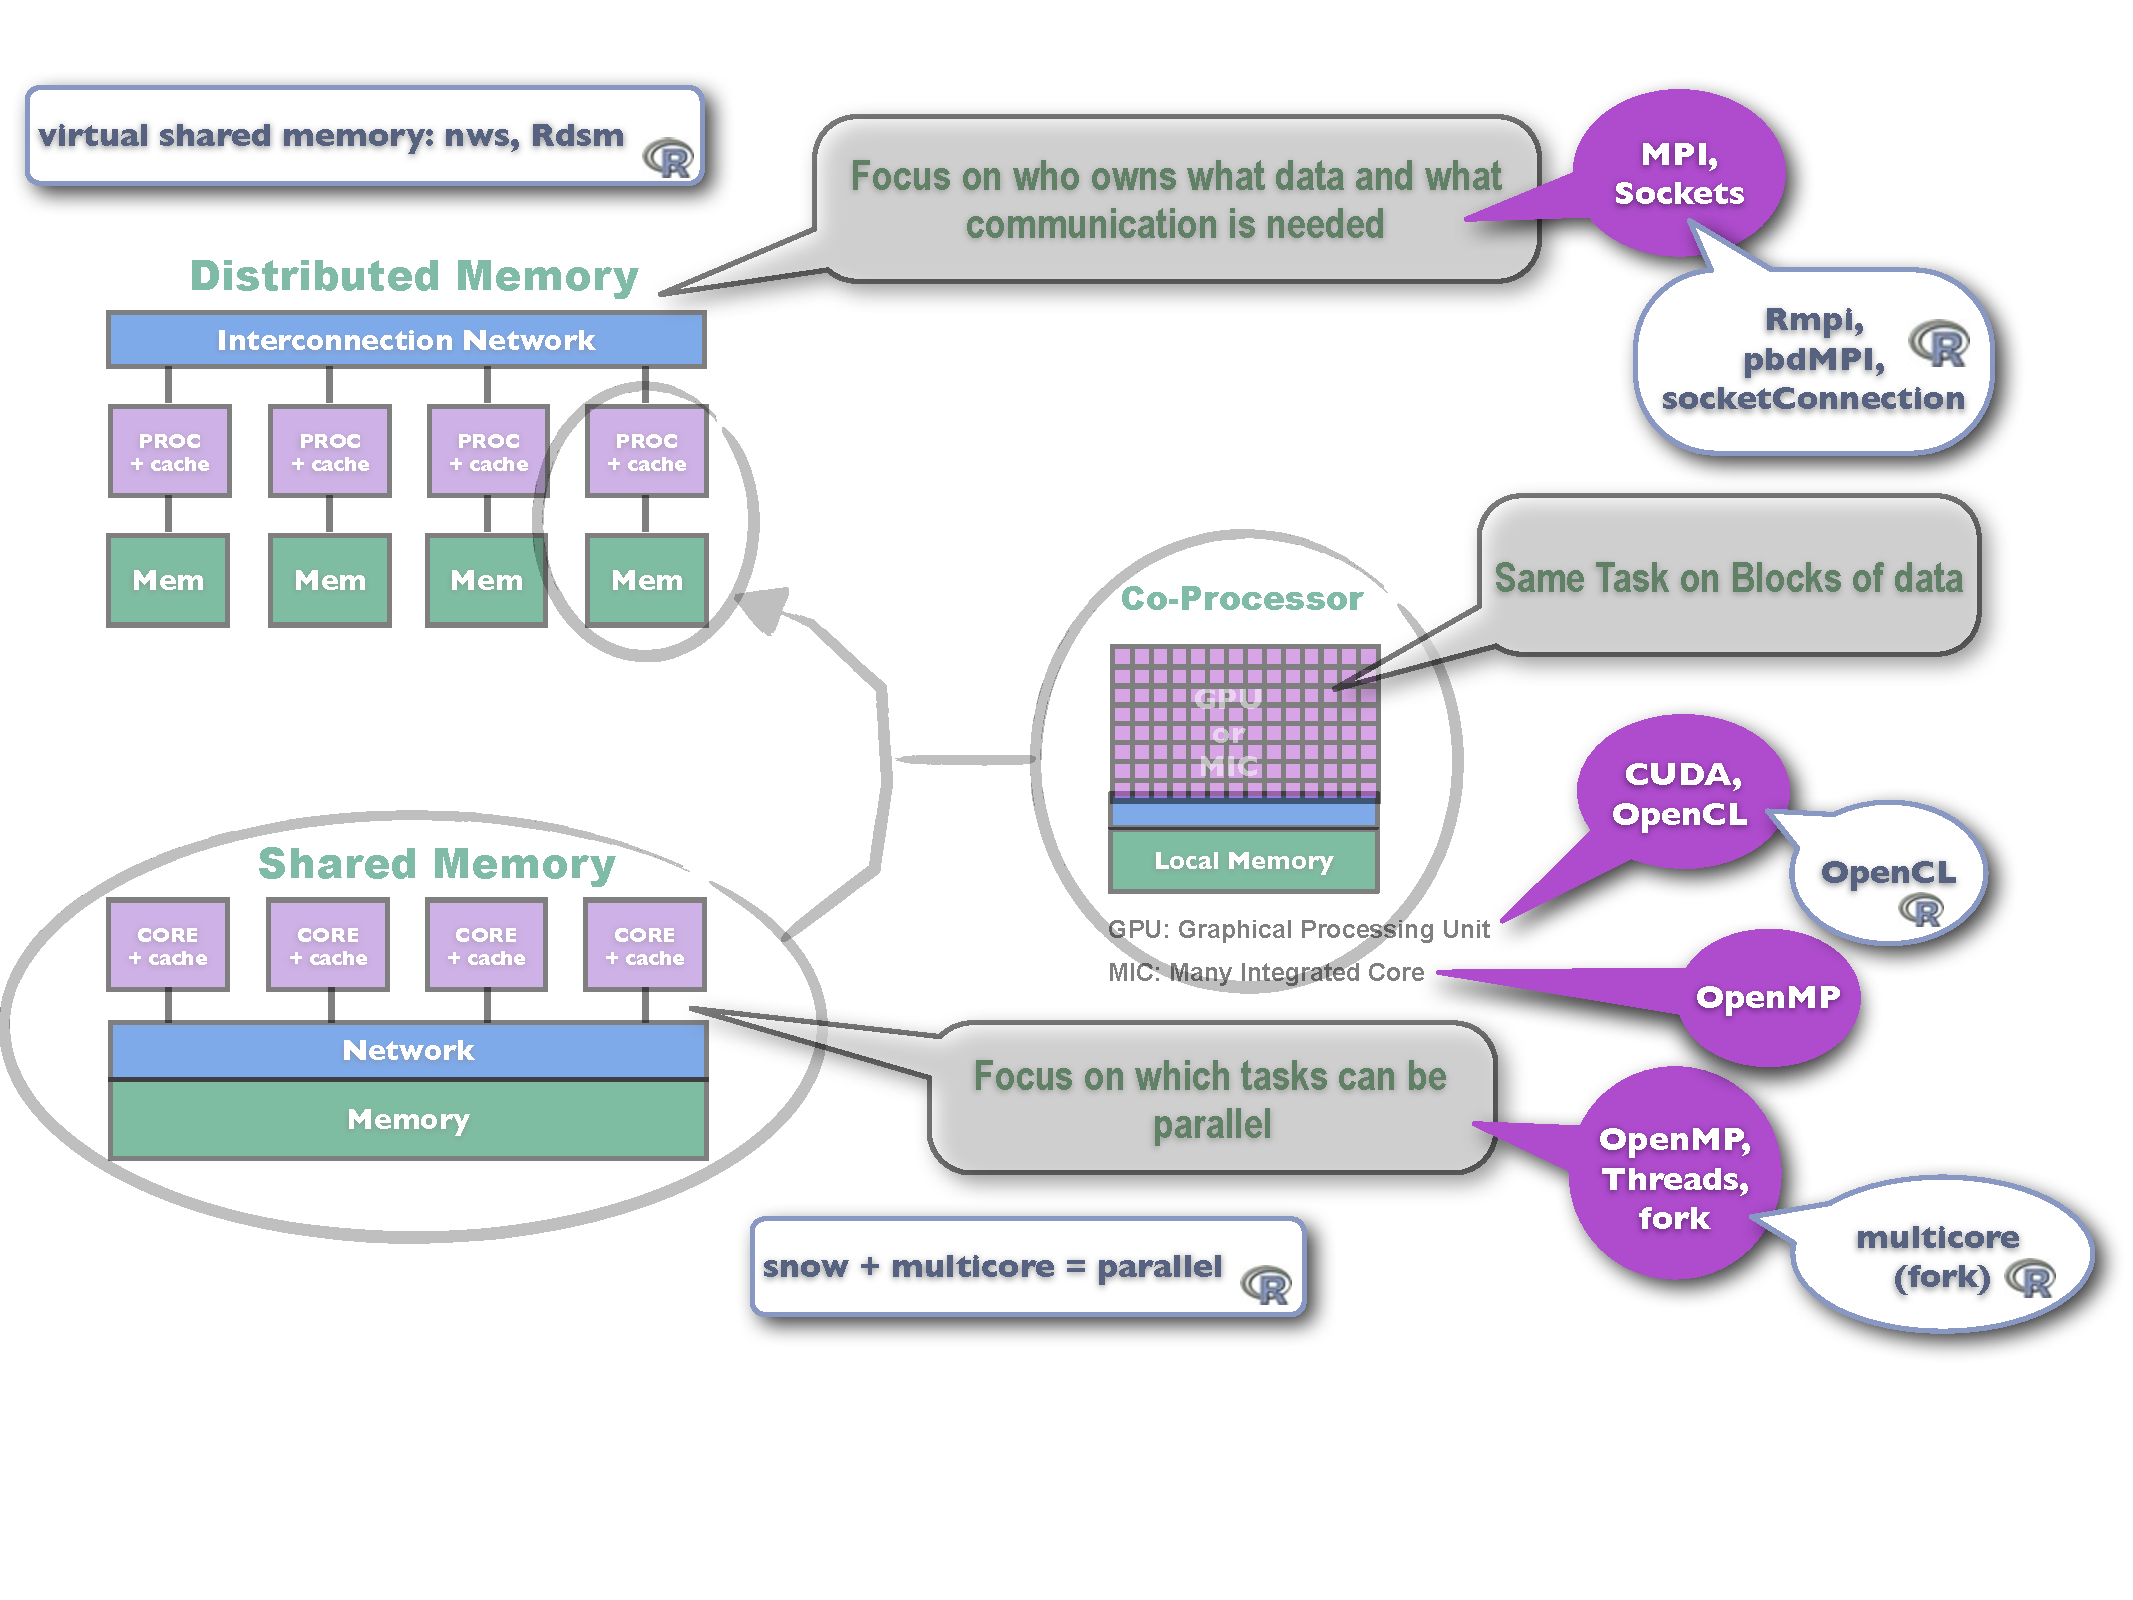
\includegraphics[width=0.95\textwidth]{../common/pics/ParallelHardware7.pdf}
\end{block}
\end{frame}

\begin{frame}
\begin{block}{30+ Years of Parallel Computing Research}
    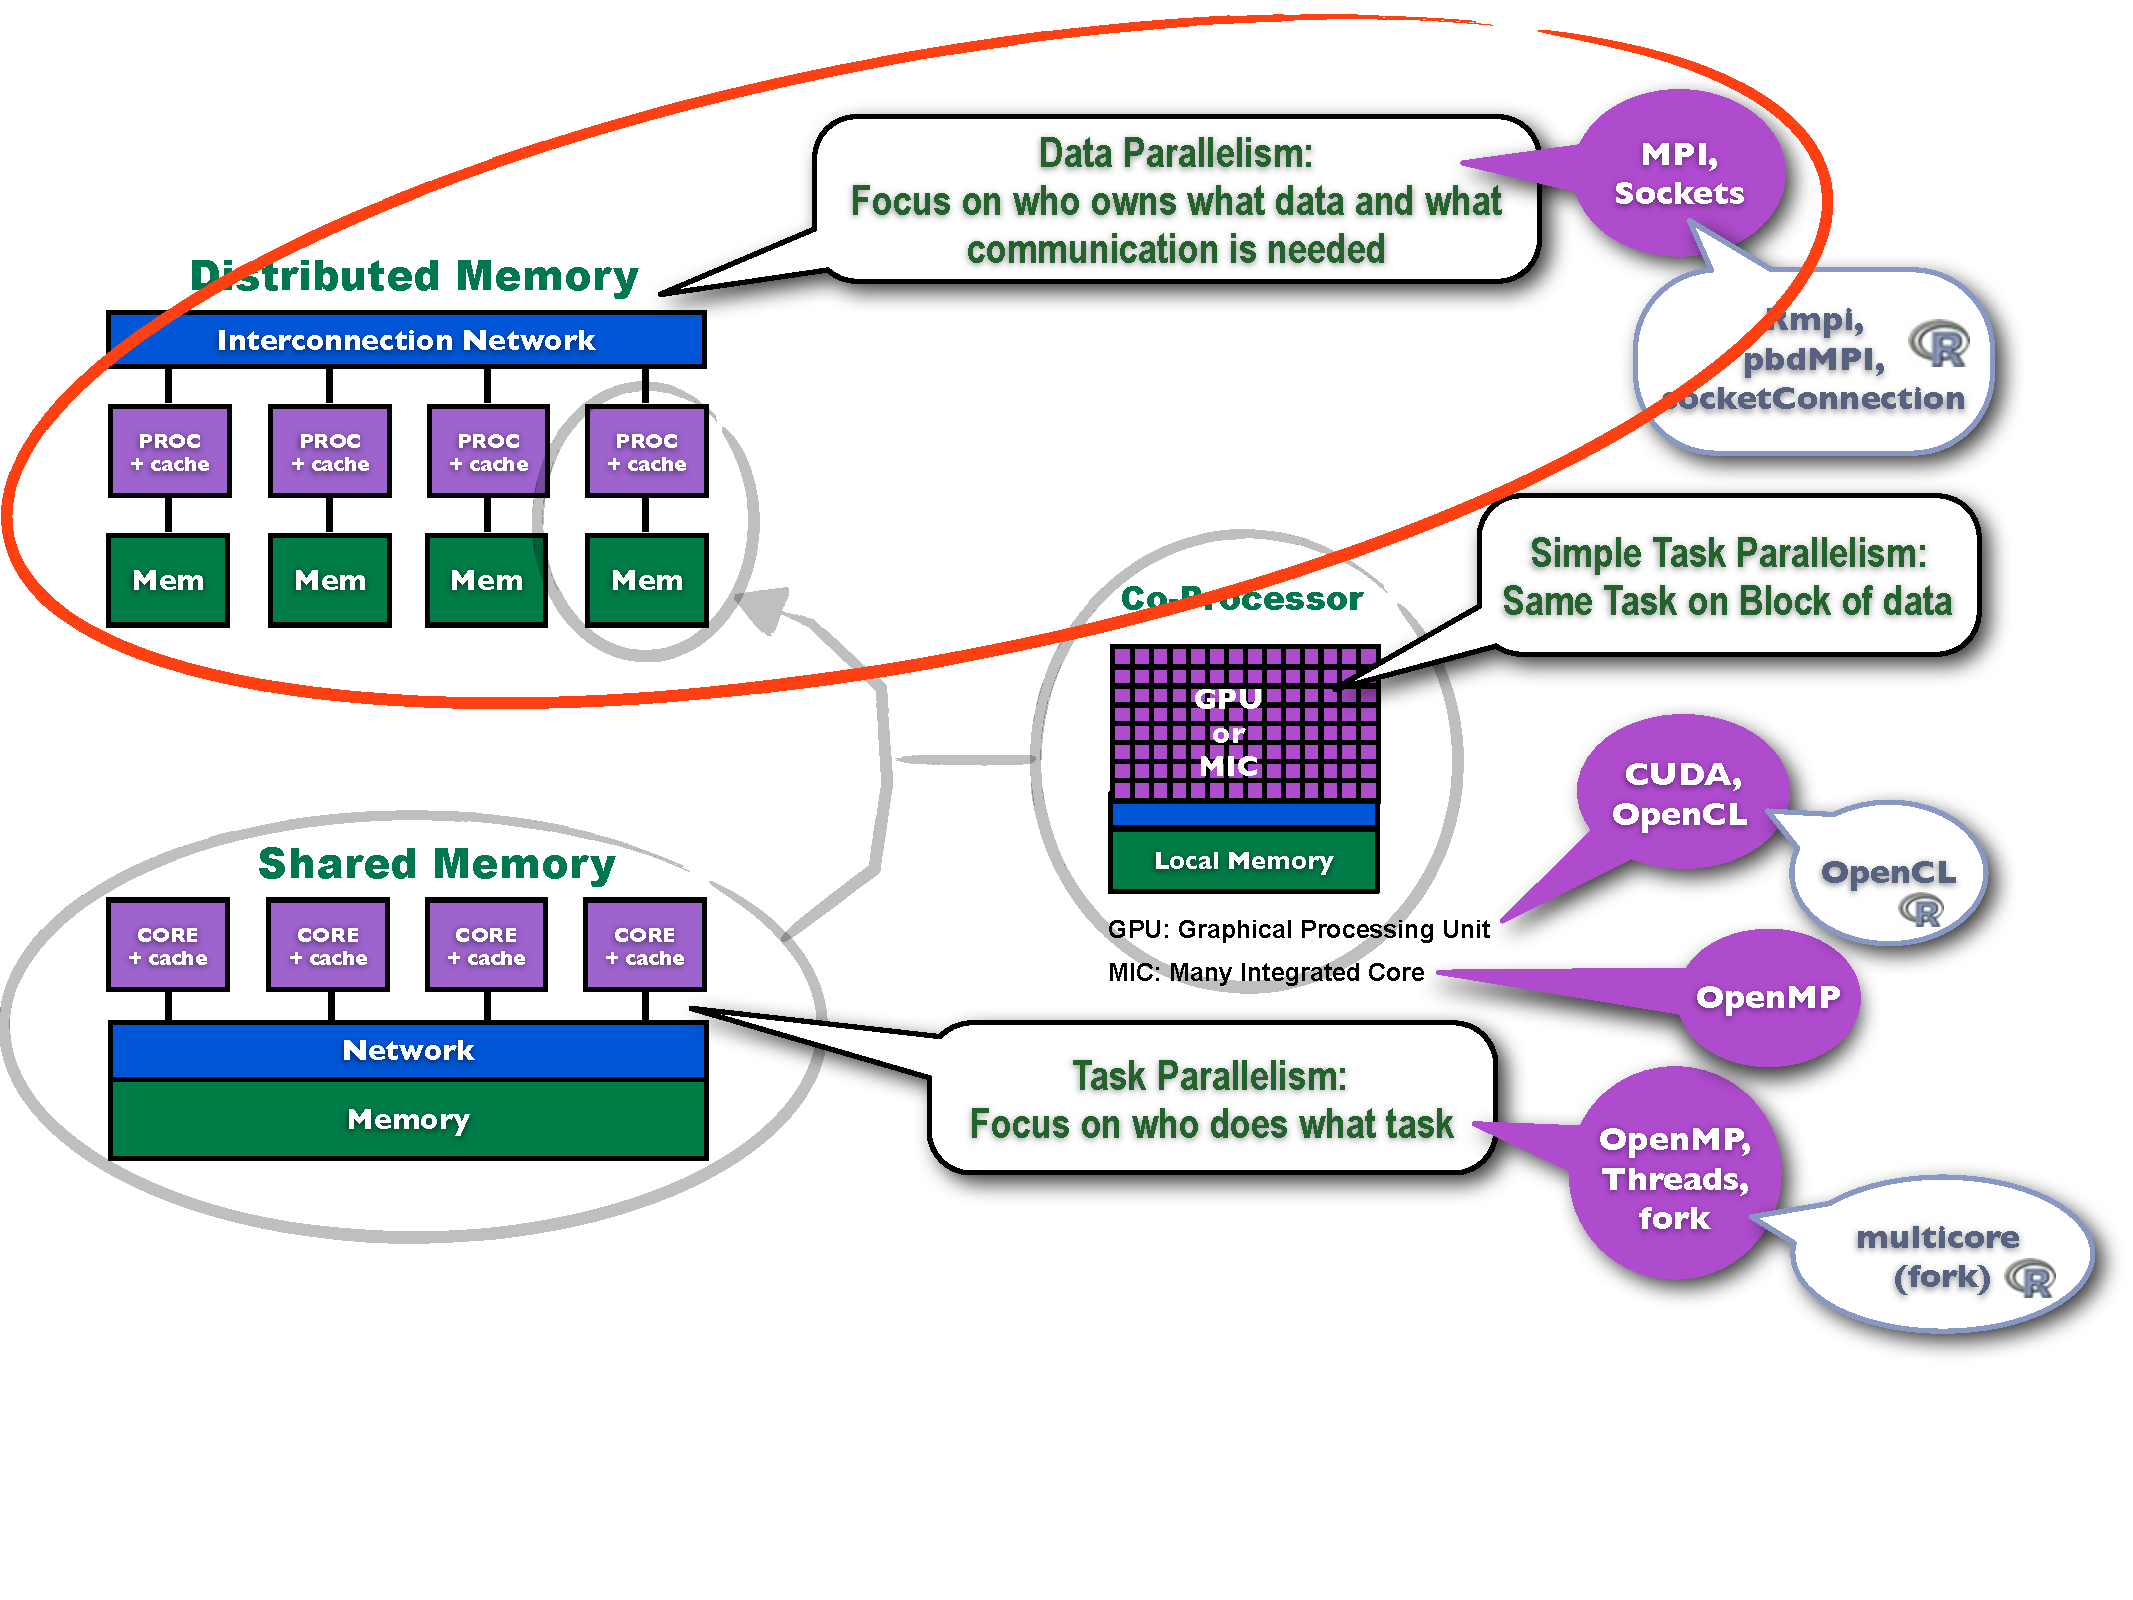
\includegraphics[width=0.95\textwidth]{../common/pics/ParallelHardware8.pdf}
\end{block}
\end{frame}

\begin{frame}
\begin{block}{Last 10 years of Advances}
    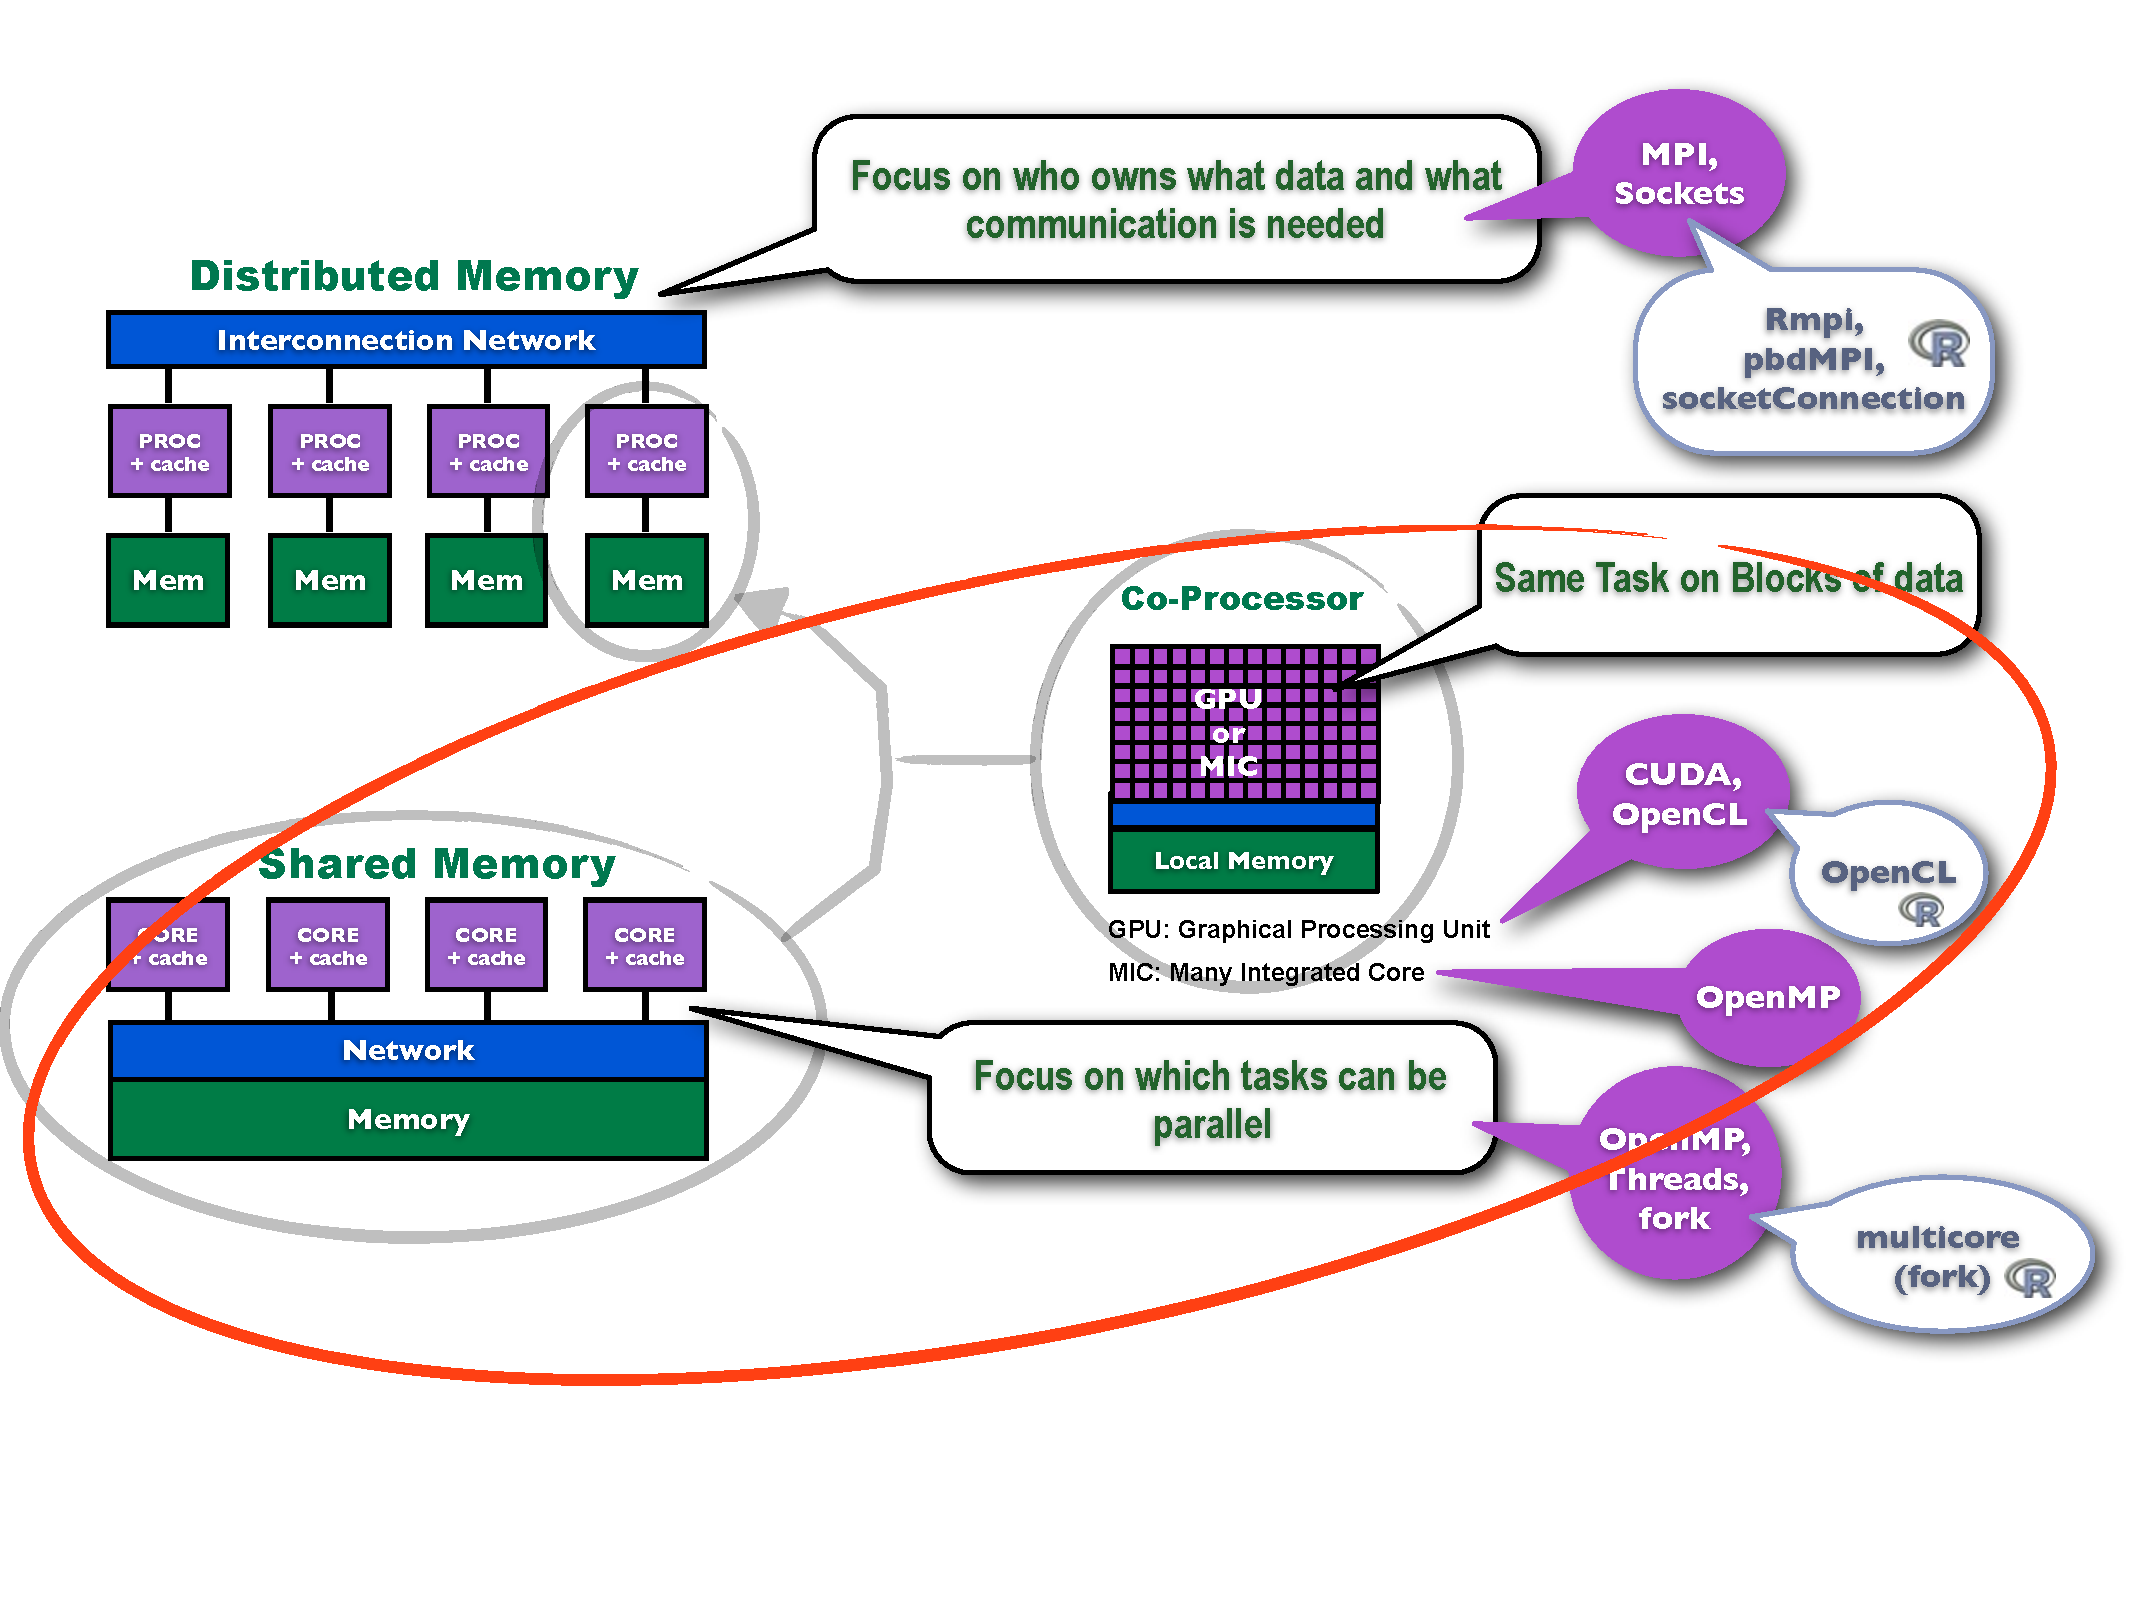
\includegraphics[width=0.95\textwidth]{../common/pics/ParallelHardware9.pdf}
\end{block}
\end{frame}

\begin{frame}
\begin{block}{Putting It All Together Challenge}
    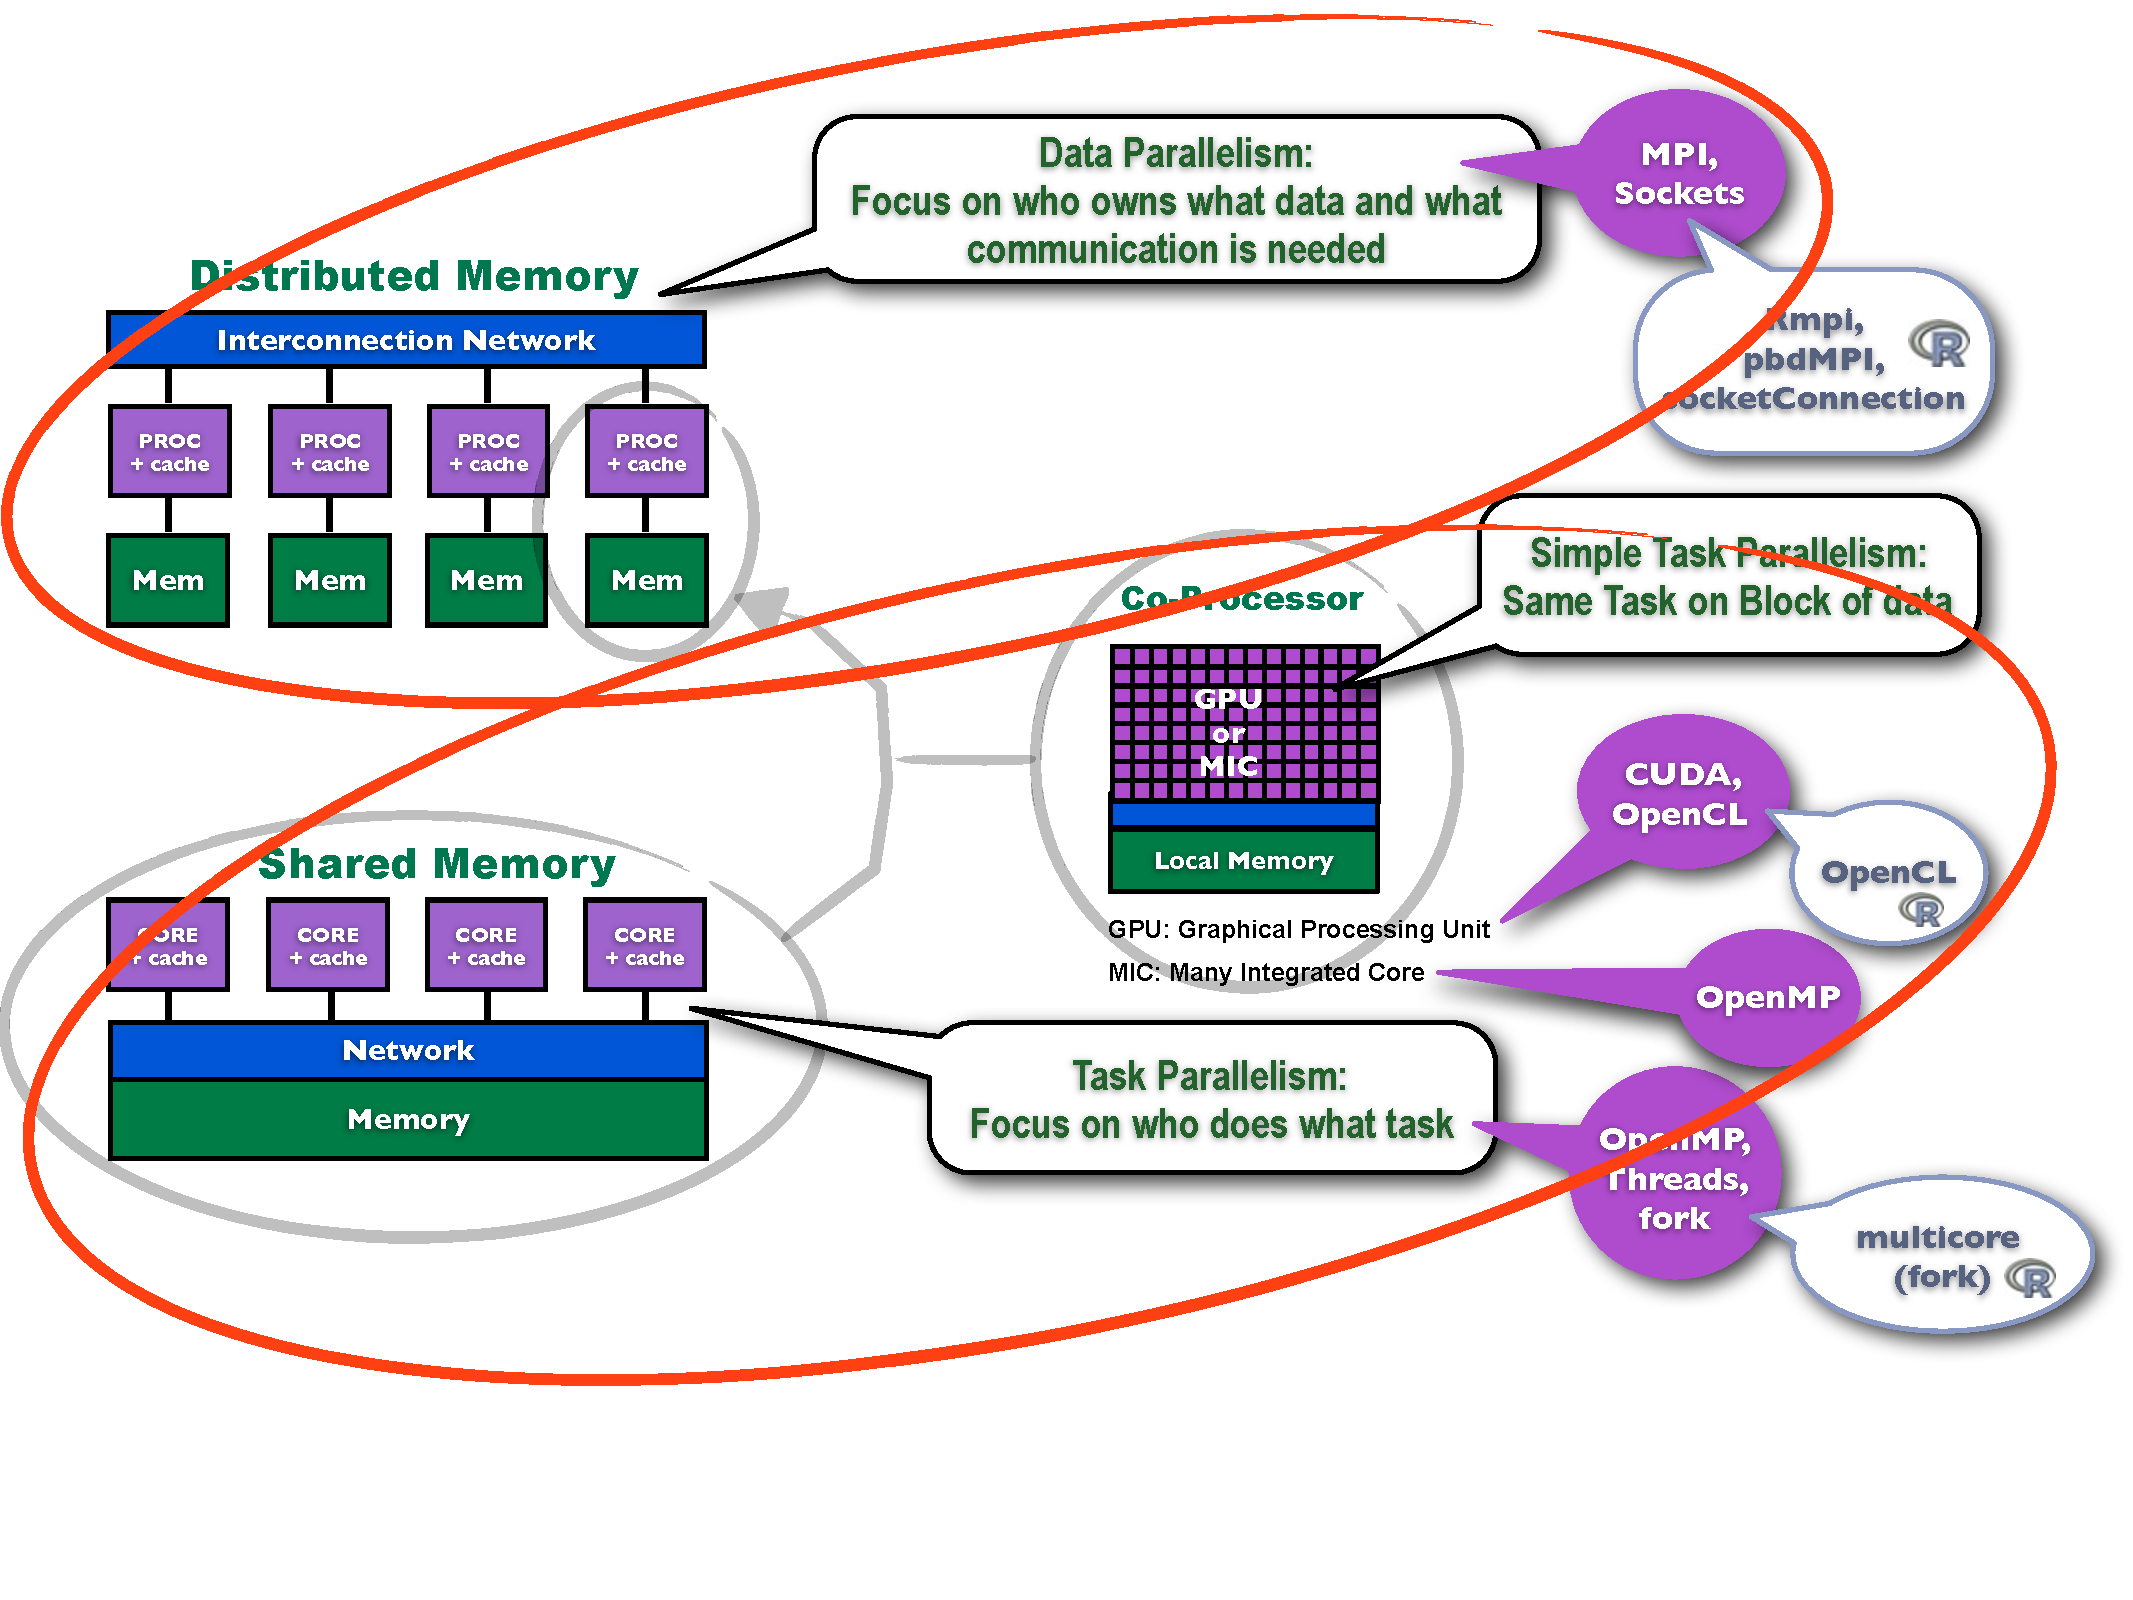
\includegraphics[width=0.95\textwidth]{../common/pics/ParallelHardware10.pdf}
\end{block}
\end{frame}

\begin{frame}
\begin{block}{pbdR Focus on Data Parallelism}
    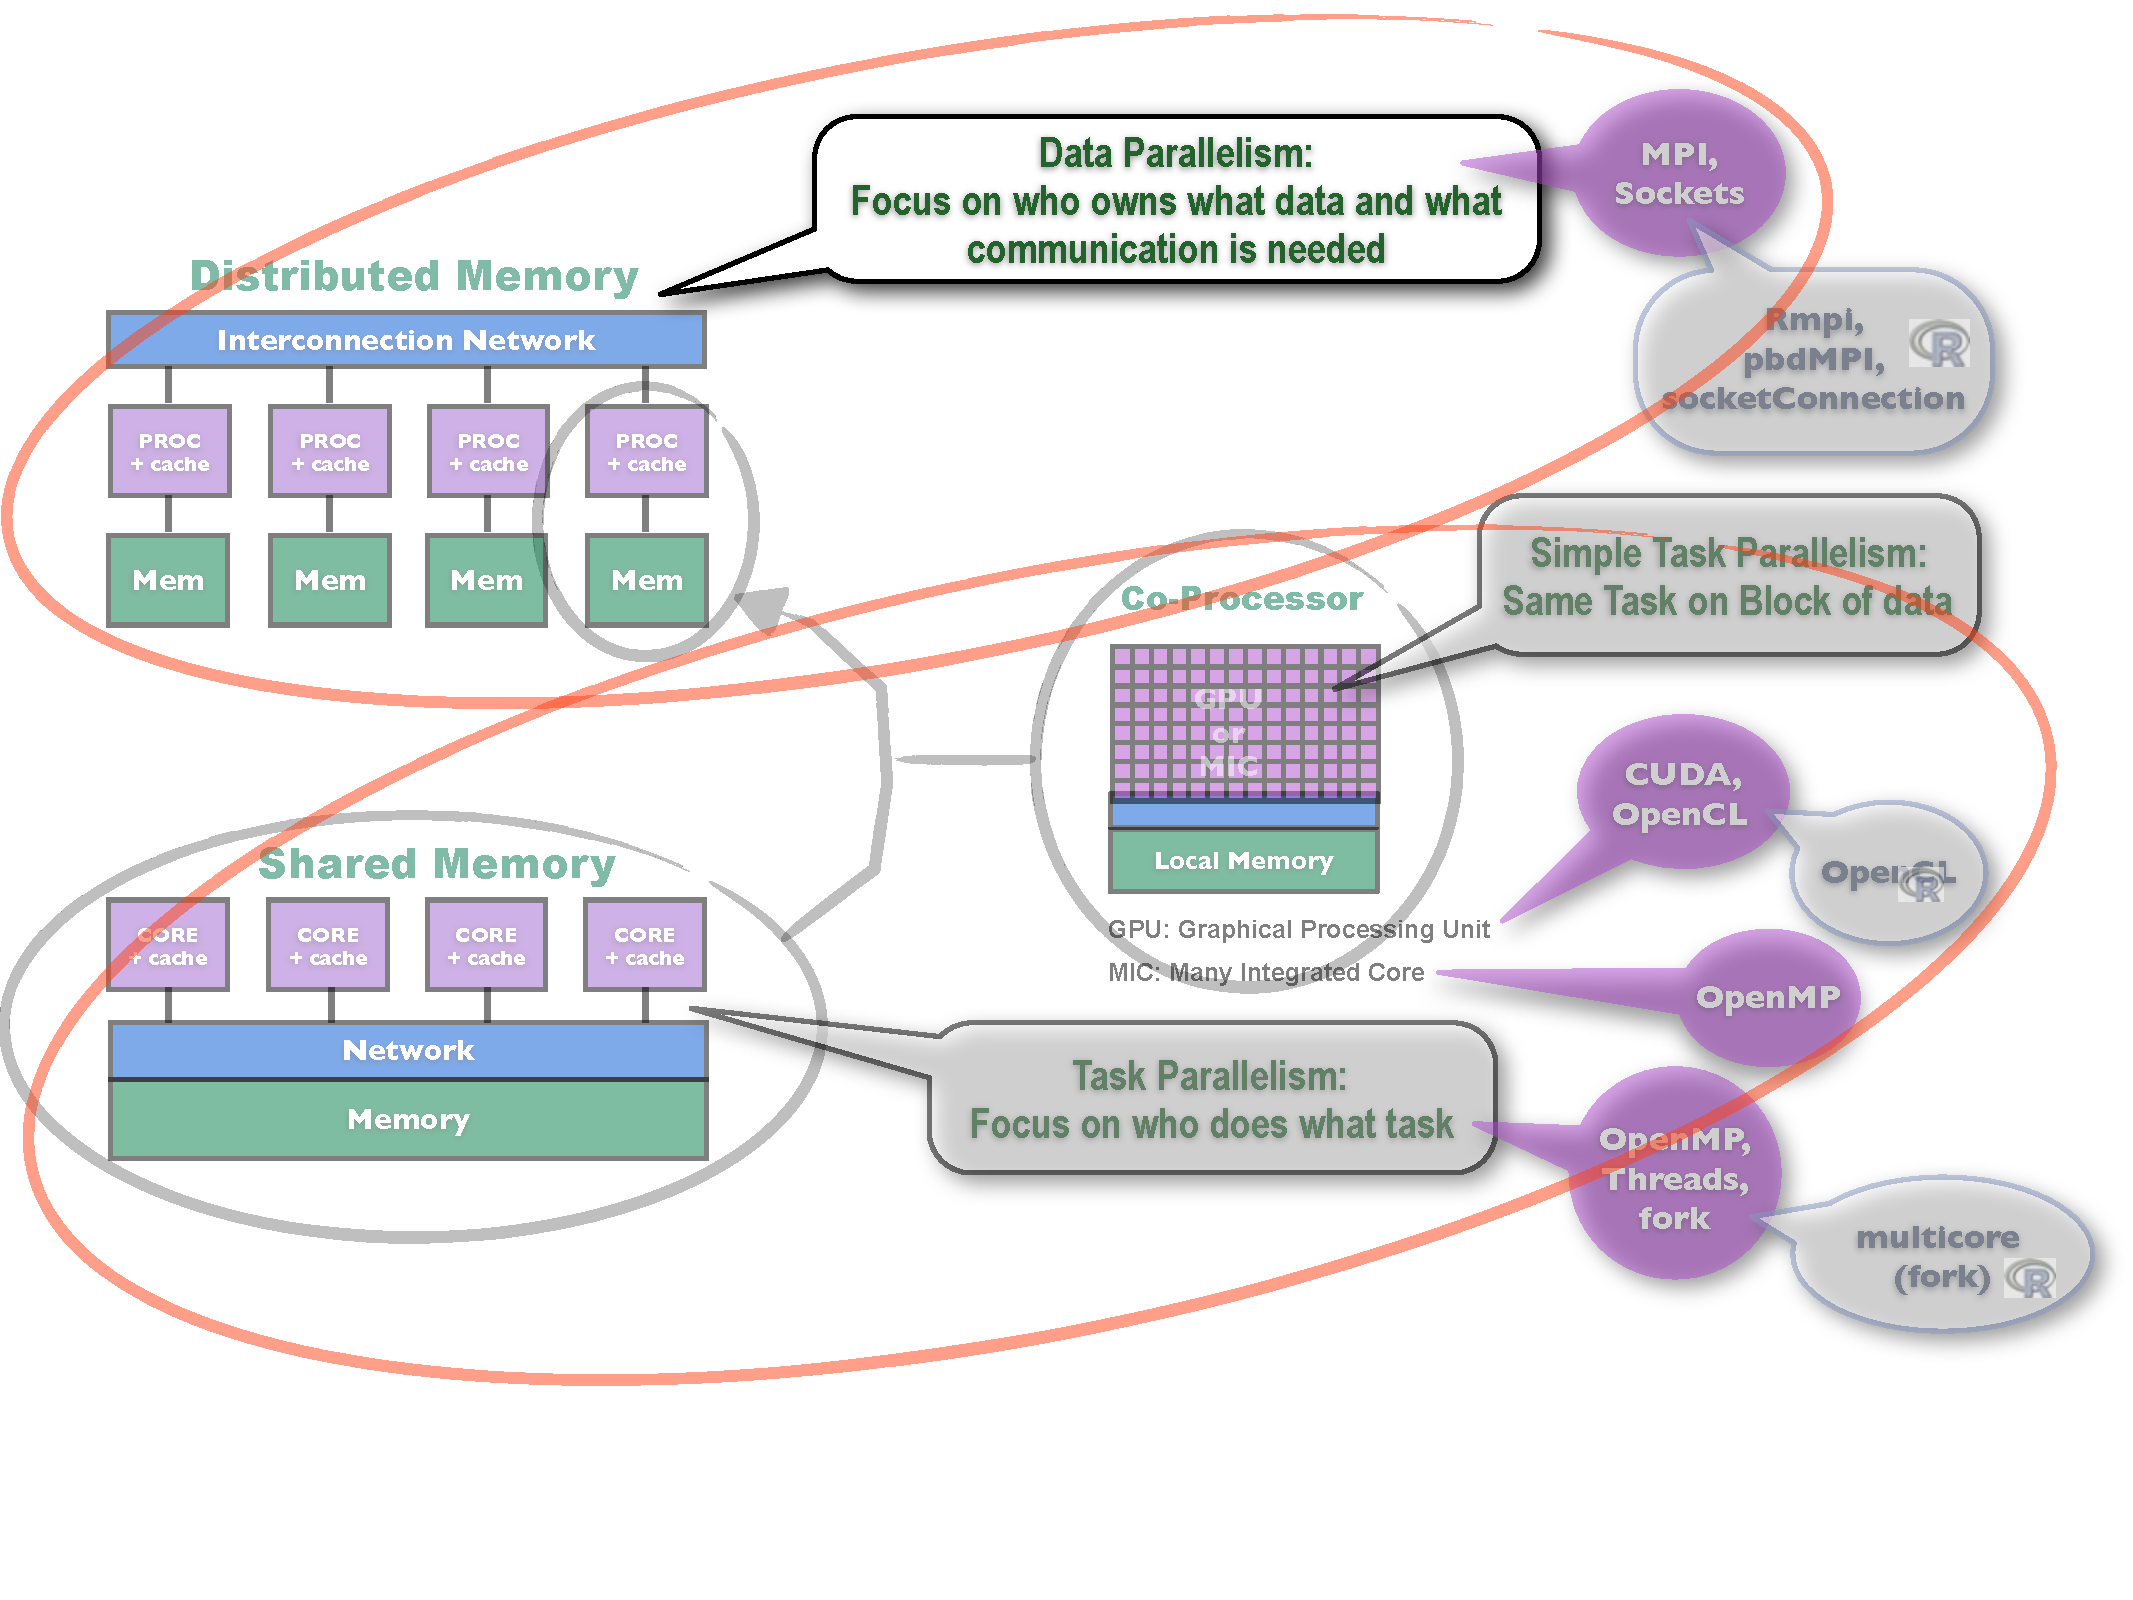
\includegraphics[width=0.95\textwidth]{../common/pics/ParallelHardware11.pdf}
\end{block}
\end{frame}

\setcounter{framenumber}{0}

\subsection{A Concise Introduction to Parallelism}

\begin{frame}
  \begin{block}{What is Parallelism?}\pause
  \begin{itemize}
    \item Doing more than one thing at a time.
    \item The simultaneous use of multiple compute resources to solve a computational problem.
  \end{itemize}
  \end{block}
\end{frame}

\begin{frame}
  \begin{block}{Parallelism}\pause
    \begin{center}
    \begin{minipage}{.46\textwidth}
    \begin{block}{\centering Serial Programming}
      \begin{center}
      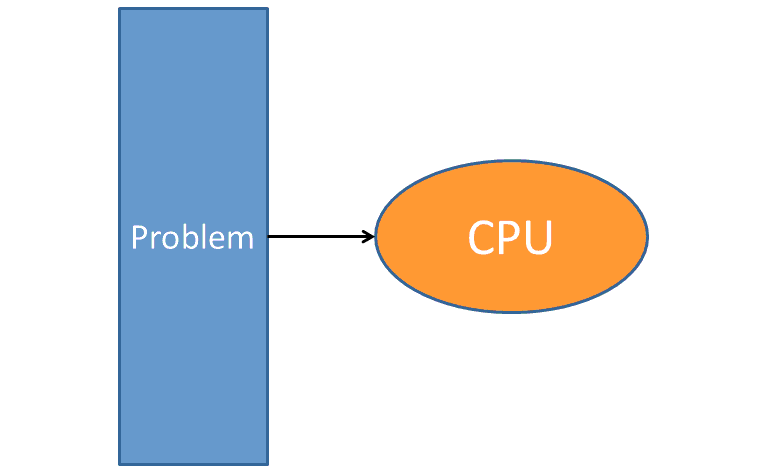
\includegraphics[width=.975\textwidth]{../common/pics/parallelism1}
      \end{center}
      \end{block}
    \end{minipage}
    \hspace{.15cm}
    \begin{minipage}{.46\textwidth}
    \begin{block}{\centering Parallel Programming}
      \begin{center}
      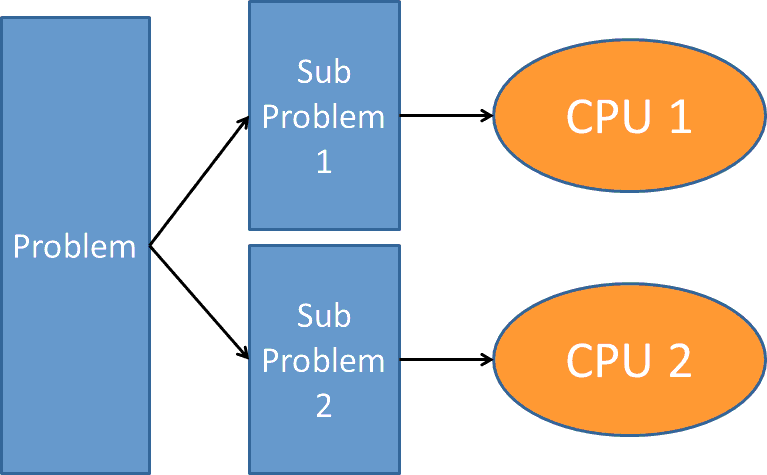
\includegraphics[width=.975\textwidth]{../common/pics/parallelism2}
      \end{center}
      \end{block}
    \end{minipage}
    \end{center}
  \end{block}
\end{frame}

\begin{frame}
  \begin{block}{Parallelism}\pause
    \begin{center}
    \begin{minipage}{.46\textwidth}
    \begin{block}{Serial Programming}
      \begin{center}
      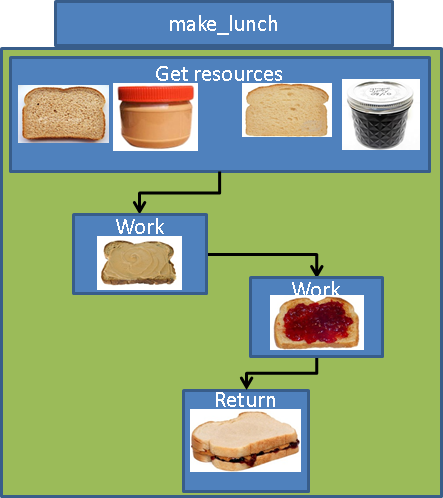
\includegraphics[width=.975\textwidth]{../common/pics/analogy_serial}
      \end{center}
      \end{block}
    \end{minipage}
    \hspace{.15cm}
    \begin{minipage}{.46\textwidth}
    \begin{block}{Parallel Programming}
      \begin{center}
      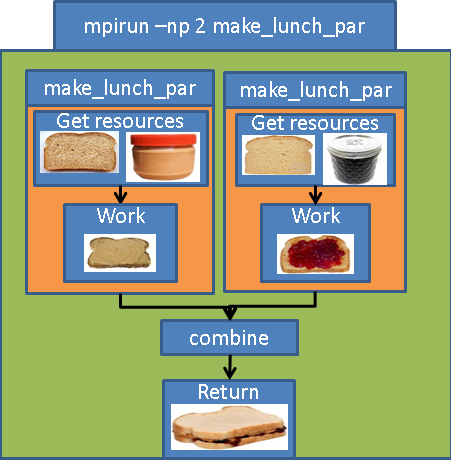
\includegraphics[height=5.45cm,width=.975\textwidth]{../common/pics/analogy_parallel}
      \end{center}
      \end{block}
    \end{minipage}
    \end{center}
  \end{block}
\end{frame}

% \begin{frame}
%   \begin{block}{What is Parallelism?}\pause
%   Broadly, \emph{doing more than one thing at a time}.\\
%     \begin{itemize}[<+-|alert@+>]
%    \item \emph{Task Parallelism}:  Many small tasks.\\
%    \emph{e.g.} Make one sandwich for each person on earth.
%    \item \emph{Data Parallelism}:  One really big task.\\
%    \emph{e.g.}  Make one sandwich so large that every person on earth could eat from it.\\
%   \end{itemize}
%   \end{block}
% \end{frame}

\begin{frame}
  \begin{block}{Kinds of Parallelism}\pause
    \begin{itemize}[<+-|alert@+>]
      \item \emph{Data Parallelism}:  Data is distributed
      \item \emph{Task Parallelism}:  Tasks are distributed
  \end{itemize}
  (This is a gross oversimplification)
  \end{block}
\end{frame}


\begin{frame}
  \begin{block}{pbdR Paradigms:  Data Parallelism}
  Data parallelism:
  \begin{itemize}[<+-|alert@+>]
   \item No one processor/node owns all the data.
   \item Processors own local pieces of a (conceptually) larger, global object
  \end{itemize}
  
  Task parallelism:
  \begin{itemize}
    \item Often involves different tasks to the same data.
  \end{itemize}
  \end{block}
\end{frame}


\begin{frame}
  \begin{block}{Data vs Task Parallelism}\pause
    \begin{center}
    \begin{minipage}{.46\textwidth}
    \begin{block}{\centering Data Parallelism}
      \begin{center}
      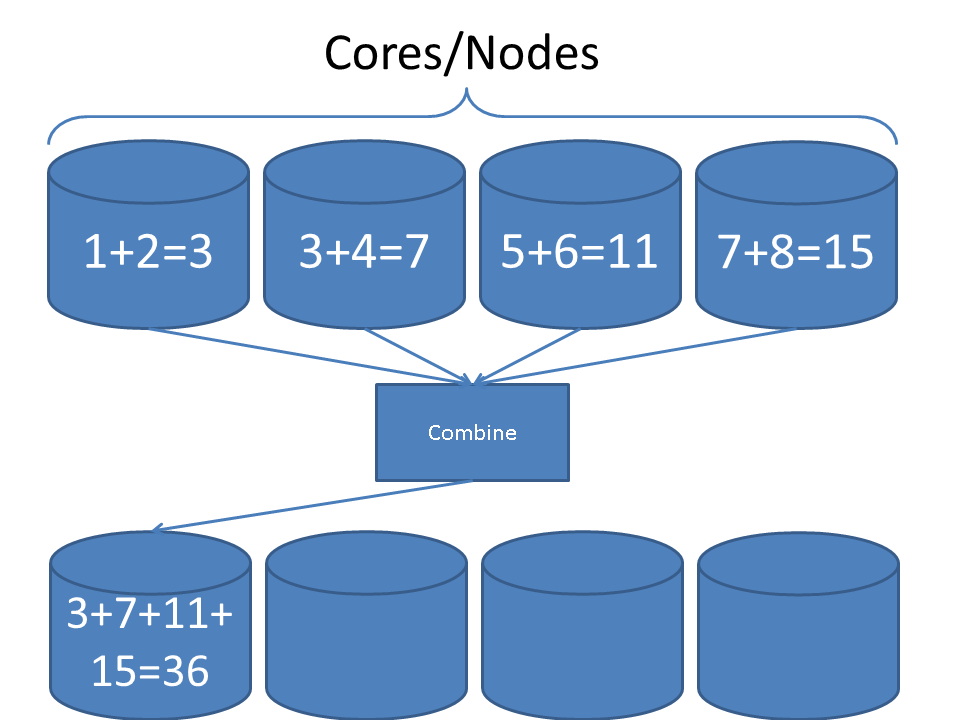
\includegraphics[width=.975\textwidth]{../common/pics/parallelism_data}
      \end{center}
      \end{block}
    \end{minipage}
    \hspace{.15cm}
    \begin{minipage}{.46\textwidth}
    \begin{block}{\centering Task Parallelism}
      \begin{center}
      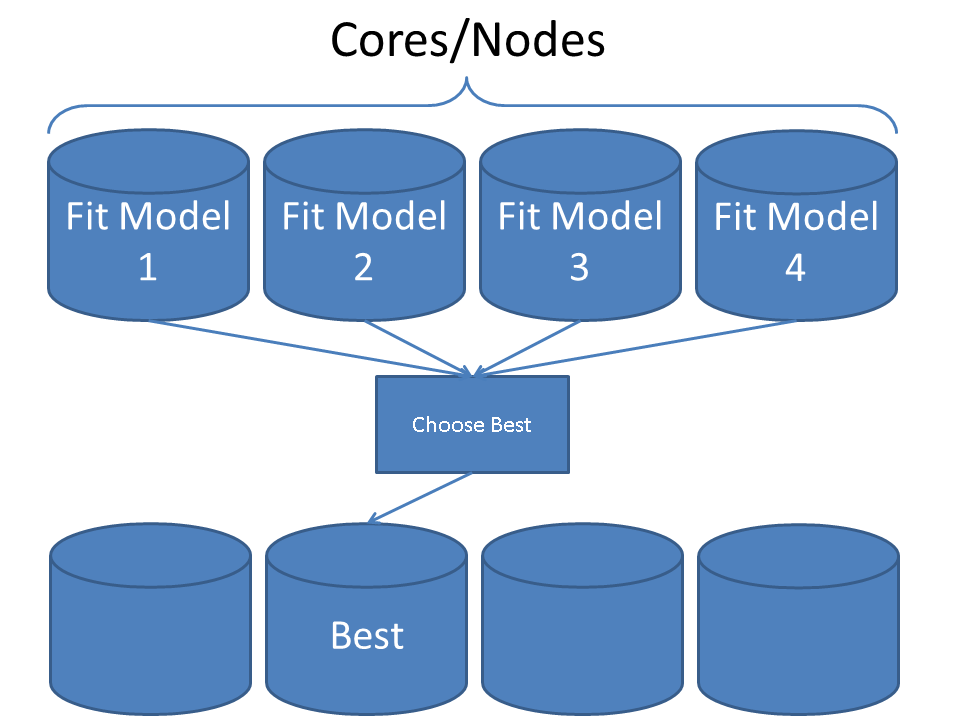
\includegraphics[width=.975\textwidth]{../common/pics/parallelism_task}
      \end{center}
      \end{block}
    \end{minipage}
    \end{center}
  \end{block}
\end{frame}




% \subsection{Common Terminology}


\begin{frame}
  \begin{block}{Parallel Programming Vocabulary:  Difficulty in Parallelism}
  \begin{enumerate}[<+-|alert@+>]
    \item \emph{Implicit parallelism}:  Parallel details hidden from user
    \item \emph{Explicit parallelism}:  Some assembly required\dots
    \item \emph{Embarrassingly Parallel}:  Also called \emph{loosely coupled}.  Obvious how to make parallel; lots of independence in computations.
    \item \emph{Tightly Coupled}:  Opposite of embarrassingly parallel; lots of dependence in computations.
  \end{enumerate}  
  \end{block}
\end{frame}


\begin{frame}
  \begin{block}{Speedup}
  \begin{itemize}
    \item \emph{Wallclock Time}:  Time of the clock on the wall from start to finish
    \item \emph{Speedup}:  unitless measure of improvement; more is better.
  \begin{align*}
   S_{n_1, n_2} =  \frac{\text{Run time for } n_1 \text{ cores}}{\text{Run time for } n_2 \text{ cores}}
  \end{align*}
  \begin{itemize}
    \item   $n_1$ is often taken to be 1
    \item In this case, comparing parallel algorithm to serial algorithm
  \end{itemize}
  \end{itemize}
  \end{block}
\end{frame}


\begin{frame}
  \begin{block}{Speedup}
   \begin{center}
    \begin{minipage}{.475\textwidth}
    \begin{block}{Good Speedup}
      \centering
      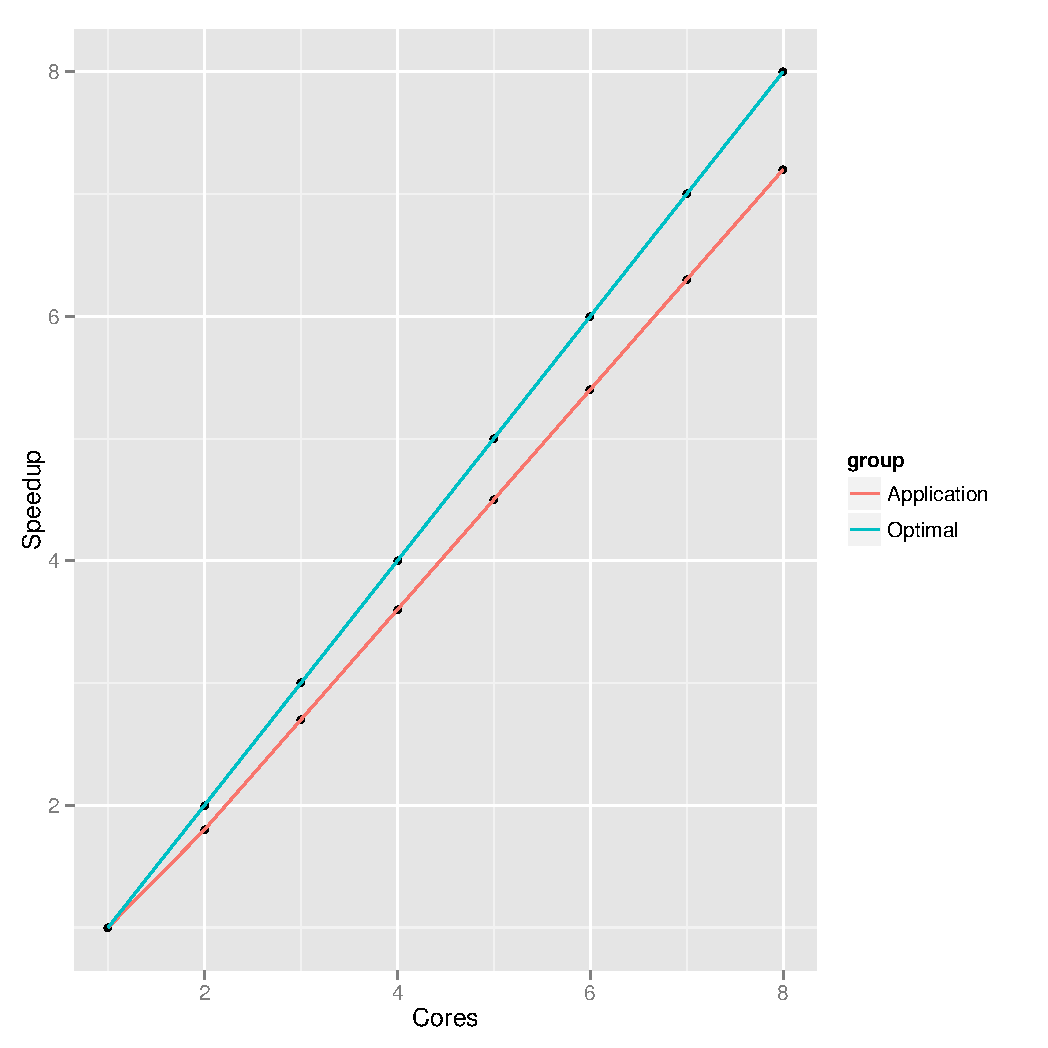
\includegraphics[width=.95\textwidth]{../common/pics/scale_good}
    \end{block}
    \end{minipage}
    \hspace{.1cm}
    \begin{minipage}{.475\textwidth}
    \begin{block}{Bad Speedup}
      \centering
      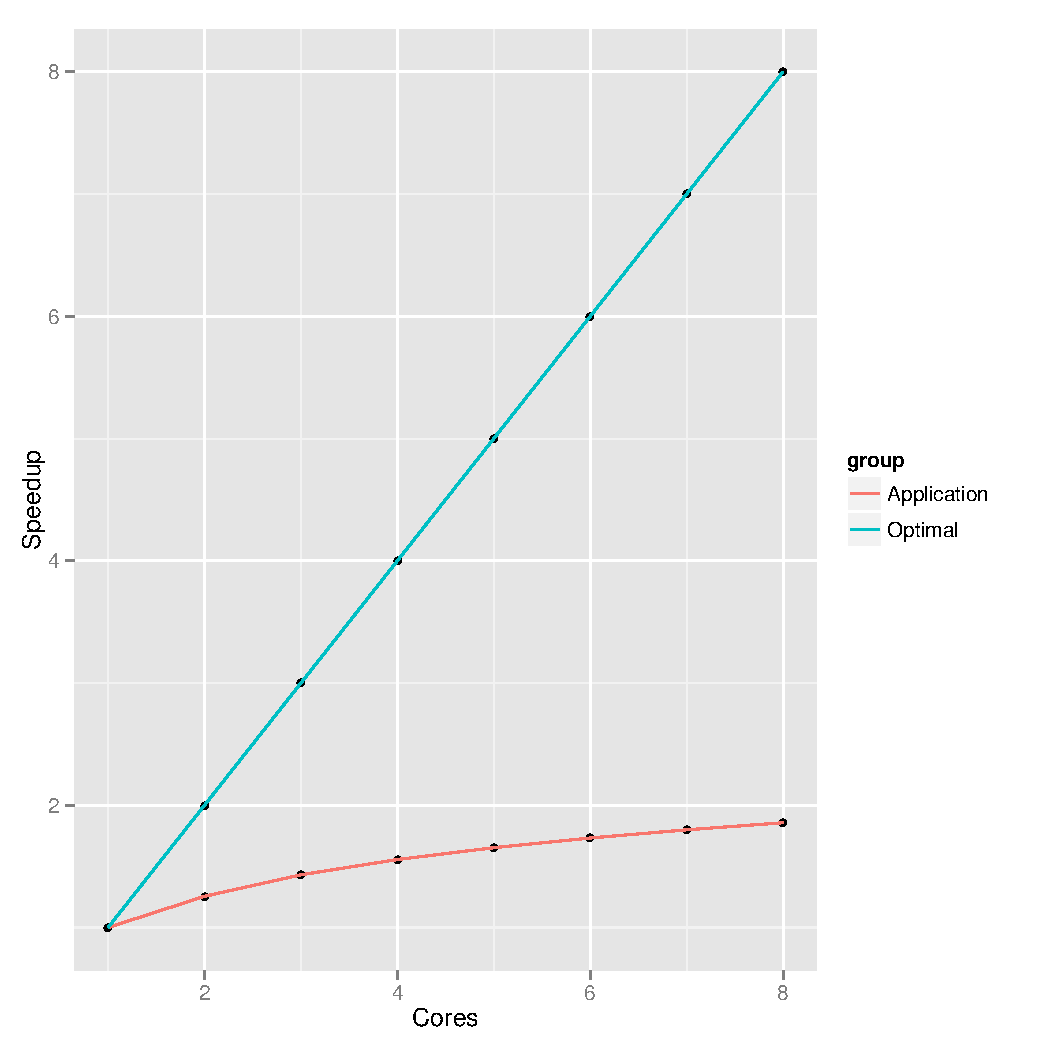
\includegraphics[width=.95\textwidth]{../common/pics/scale_bad}
    \end{block}
    \end{minipage}
    \end{center}
    \end{block}
\end{frame}


\begin{frame}
  \begin{block}{Recall: Shared and Distributed Memory Machines}
   \begin{center}
    \begin{minipage}{.475\textwidth}
    \begin{block}{Shared Memory}
     Direct access to read/change memory (one node) \vspace{.3cm} \ 
      \begin{center}
      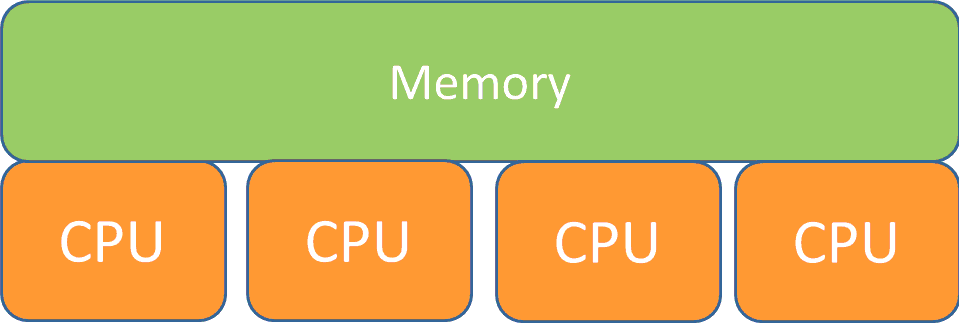
\includegraphics[width=.95\textwidth]{../common/pics/arch_shared}
      \end{center}
      \vspace{.3cm} \
    \end{block}
    \end{minipage}
    \hspace{.1cm}
    \begin{minipage}{.475\textwidth}
    \begin{block}{Distributed}
    No direct access to read/change memory (many nodes); requires communication
      \begin{center}
      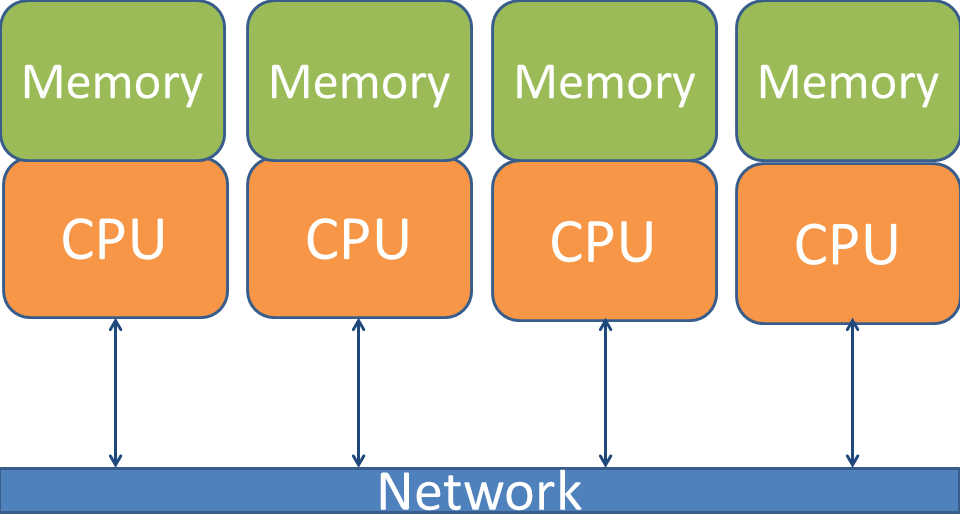
\includegraphics[width=.95\textwidth]{../common/pics/arch_distributed}
      \end{center}
    \end{block}
    \end{minipage}
    \end{center}
    \end{block}
\end{frame}


\begin{frame}
  \begin{block}{Shared and Distributed Memory Machines}
   \begin{center}
    \begin{minipage}[t]{.47\textwidth}
    \begin{block}{Shared Memory Machines}
    \begin{center}
    Thousands of cores\\[.2cm]
    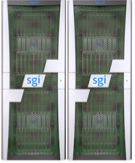
\includegraphics[scale=.65]{../common/pics/nautilus}\\
    {\tiny \emph{Nautilus}, University of Tennessee\\1024 cores \\4 TB RAM\\}
    \end{center}
    \end{block}
    \end{minipage}
    \hspace{.1cm}
    \begin{minipage}[t]{.47\textwidth}
    \begin{block}{Distributed Memory Machines}
    \begin{center}
    Hundreds of thousands of cores\\[.2cm]
    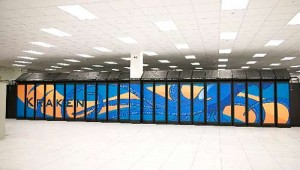
\includegraphics[width=.95\textwidth]{../common/pics/kraken}\\
    {\tiny \emph{Kraken}, University of Tennessee\\ 112,896 cores \\147 TB RAM\\}
    \end{center}
    \end{block}
    \end{minipage}
    \end{center}
    \end{block}
\end{frame}




\subsection{R and Parallelism}


\begin{frame}
%  \addtocounter{framenumber}{-1}
  \begin{block}{R and Parallelism}\pause
  What about R?
  \end{block}
\end{frame}

\begin{frame}
%  \addtocounter{framenumber}{-1}
  \begin{block}{Problems with Serial R}\pause
  \begin{enumerate}[<+-|alert@+>]
    \item Slow.
    \item If you don't know what you're doing, it's \emph{really} slow.
    \item Performance improvements usually for small machines.
    \item Very ram intensive.
  \end{enumerate}
  \end{block}
\end{frame}


\begin{frame}
  \begin{block}{Why We Need Parallelism}\pause
    \begin{enumerate}[<+-|alert@+>]
      \item Saves compute time.
      \item Data size is skyrocketing.
      \item Necessary for many problems.
      \item Its necessity is coming.
      \item \emph{It's really cool.}
  \end{enumerate}
  \end{block}
\end{frame}

\begin{frame}
  \begin{block}{Recall: Parallel R Packages}
   \begin{center}
    \begin{minipage}{.45\textwidth}
    \begin{block}{Shared Memory}
      \begin{enumerate}[<+-|alert@+>]
        \item \pkg{foreach}
        \item \pkg{parallel}
        \item \pkg{snow}
        \item \pkg{multicore}
      \end{enumerate}
    \end{block}
    \end{minipage}
    \hspace{.2cm}
    \begin{minipage}{.45\textwidth}
    \begin{block}{Distributed}
      \begin{enumerate}[<+-|alert@+>]
        \item \pkg{Rmpi}
        \item R+Hadoop
        \item \pkg{pbdR}
      \end{enumerate}
    \end{block}
    \end{minipage}
    \end{center}
    (and others\dots)
    \end{block}
\end{frame}



\begin{frame}[shrink]
  \begin{block}{R and Parallelism}
    The solution to many of R's problems is parallelism.  However \dots\vspace{-.4cm}
   \begin{center}
    \begin{minipage}[t]{.95\textwidth}
    \begin{block}{\centering What we have}
      \begin{enumerate}[<+-|alert@+>]
        \item Mostly serial.
        \item Mostly not distributed
        \item Data parallelism mostly explicit
      \end{enumerate}
    \end{block}
    \end{minipage}
    \\\pause
    \begin{minipage}[t]{.95\textwidth}
    \begin{block}{\centering What we want}
      \begin{enumerate}[<+-|alert@+>]
        \item Mostly parallel.
        \item Mostly distributed.
        \item Mostly implicit.
      \end{enumerate}
    \end{block}
    \end{minipage}
    \end{center}
    \end{block}
\end{frame}



\begin{frame}
  \begin{block}{R and Parallelism}
    Likewise, the HPC community is looking for high-level languages for data\dots
    \end{block}
\end{frame}

